\part{Introduction}

\chapter{Introduction}

What has been one of the main dangers humanity has faced throughout its history? The first answers that can be given are war or climate change, but there is another great threat that has severely affected the lives of almost all human populations over time: diseases and epidemics. There were no periods - not in the past, nor nowadays - when illnesses didn't influence human lives. 

Looking at the past, the consequences of epidemics on the population were worse than today mostly because of the lack of knowledge about medical science and the poor hygienic conditions. During the bubonic plague of the 14th century, for example, 25 million deaths were reported in Europe out of a population of 100 million. The pandemic also triggered social unrest: Jews were considered responsible for the illness spread and they began to be persecuted.

\begin{figure}[]
	\centering
	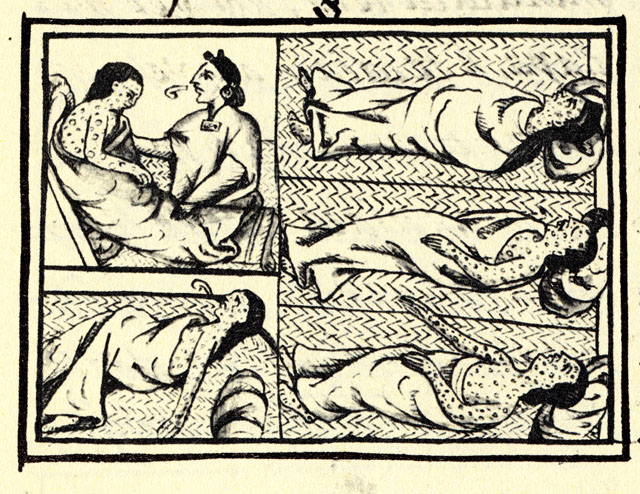
\includegraphics[width=0.4\linewidth]{0_introduction/images_introduction/FlorentineCodex_smallpox}
	\caption[Smallpox on native Americans]{Representation of smallpox disease on the Mexican population in the $XIV$ century. Figure from the Florentine Codex \cite{Sahagun1965}. }
	\label{fig:florentinecodexsmallpox}
\end{figure}

In addition, during the course of the Americas' colonization, the diseases imported by the Europeans were one of the main causes of the genocide of the local population, largely contributing to their defeat against the Spanish conquistadores. In fact, diseases like smallpox and cholera were unknown in these countries and native Americans had no antibodies to contrast them. 
Other important epidemics, famous for their consequences, were Spanish influenza, Smallpox, Typhus, HIV/AIDS, and the more recent COVID-19. 
It is straightforward to notice the effect that diseases have on our lives.

The development of modern medicine and hygiene contributed to enhancing the quality of life. An example of this is that only in the last three centuries and especially in the most economical developed countries, a significant increase in life expectancy has been observed \cite{Anderson_82}.
This increase is also happening in poorer regions, such as Sub-Saharan Africa. Although their current life expectancy is lower than that of wealthier countries, recent research \cite{Vollset_2024} predicts a significant rise over the next 30 years. This study also forecasts that this trend will lead to a global convergence in life expectancy between now and 2050.
The most plausible explanation for this future prediction is that improvements in healthcare levels lead to changes in the causes of mortality as nations' wealth increases. In poorer regions, the primary causes of death are communicable, maternal, neonatal, and nutritional diseases, whereas in more developed and wealthier countries, non-communicable diseases like cancer and cardiovascular conditions become the main causes of death \cite{CITARE_DEVO_RITROVARE_LA_FONTE}.

However, despite rising life expectancy, epidemics continue to be one of the most significant threats to populations. In fact, there was a notable increase in the frequency and magnitude of reported epidemics during the 19th and 20th centuries \cite{Anderson_82}. This makes it essential to develop effective policies to control and mitigate their impact, requiring coordinated implementation by countries within the same macro-region.
\begin{figure}[h]
	\centering
	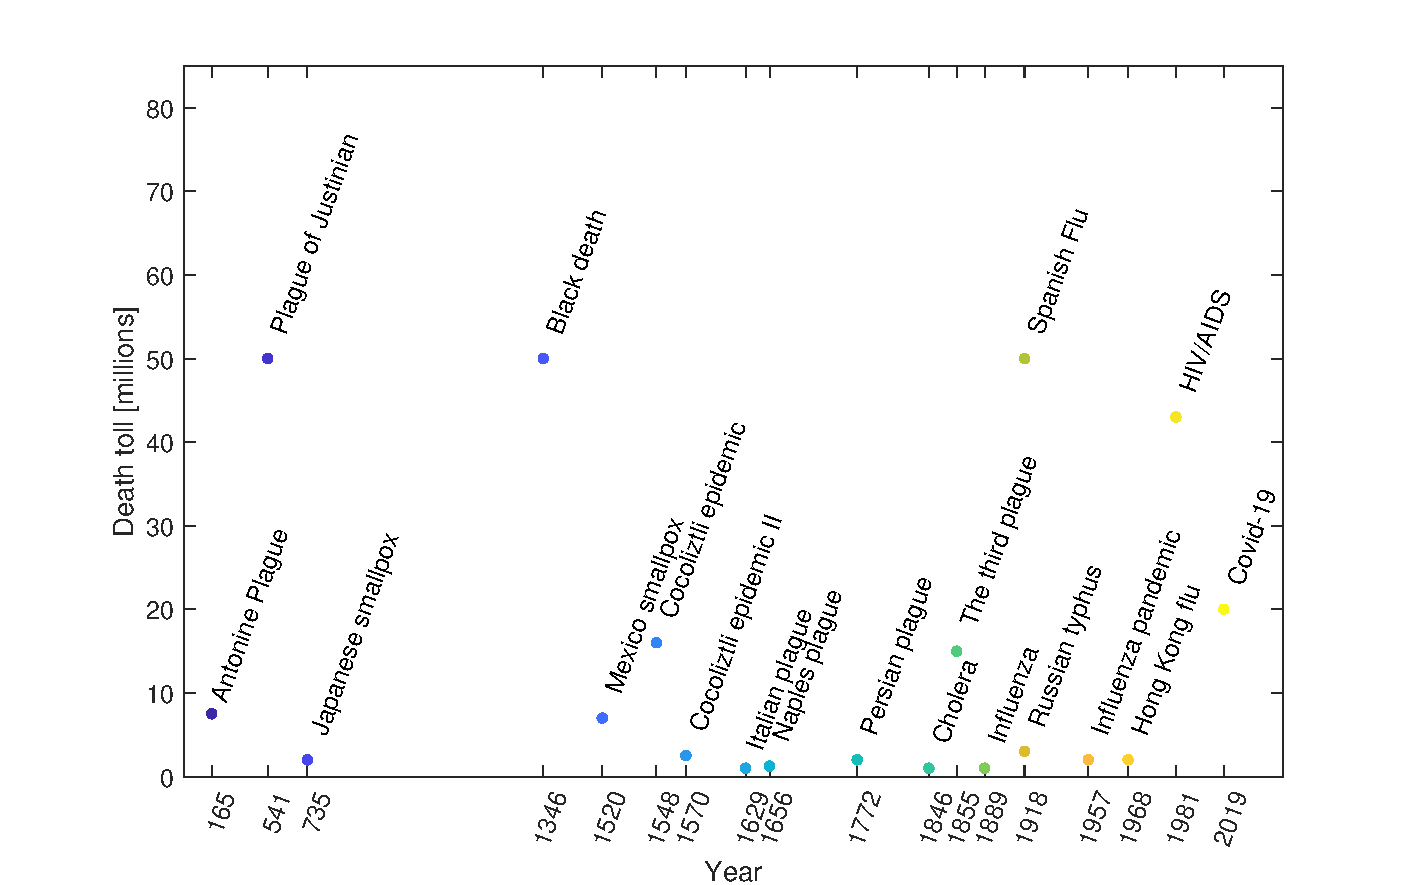
\includegraphics[width=0.85\linewidth]{0_introduction/images_introduction/worst_epidemic}
	\caption[Epidemic distribution in time]{A graphical representation of the epidemic distribution over the years and of their associated death toll. It is observable how there is an increment in the number of these event in the last three centuries. Data extracted from \cite{owid_historical_pandemics,wiki_pandemics}}
	\label{fig:worstepidemic}
\end{figure}

Figure \ref{fig:worstepidemic} highlights this trend. Although it becomes increasingly difficult to obtain reliable information about disease outbreaks the further back in time one goes, epidemics remain a tangible and present threat. This underscores the need for attention and action in shaping health policies that effectively address these dangers.
However, health status is not the only factor impacted by disease. Illness can profoundly alter relationships, work, and social life, leading to a deterioration in overall social well-being as well \cite{Yang_2020}. 
There is also an economic cost associated with the cure necessary to be healed. Only in a few nations worldwide, is treatment covered free of charge by the state. In the majority, being ill can result in having to sustain high costs, causing people to go into debt or not take care \cite{esteban_2017, Barlow2021}. 
All these effects sum together and influence how populations behave when facing an epidemic. What are the consequences of adopting a certain behavior during a disease outbreak? It's a crucial question and can help to understand how to develop more efficient policies for contrasting epidemics. It is also the question that represents the first objective of study for the present work: How can a multidisciplinary model be developed that integrates elements from both social and epidemiological aspects to provide some insights into their mutual influence during the spread of a disease?
\\
\newline
Taking a step back, it's important to understand why epidemic models are crucial and what this field of research entails.
When a new disease emerges, the primary objective is to develop a defense against it. This begins with an epidemiological investigation to understand the disease's origin, the biological mechanisms behind its spread, and its resistance to existing drugs. The goal of this investigation is to gather all available information and understand the unfolding situation.
The next crucial step involves studying the dynamics of the disease and developing a predictive model for its evolution. This process requires understanding and estimating various parameters associated with the disease, including the transmission mechanisms within the population, the reproductive rate of the infectious agent, the acquisition and persistence of immunity, and the contagion mechanism.
Creating a reliable model is not only scientifically valuable but also serves as a powerful tool for stakeholders, helping to formulate effective policies during a pandemic emergency. Theoretical epidemiology aims to provide insights and policy recommendations in this context. Furthermore, data acquisition and analysis are essential for statistically modeling epidemic coefficients. 
Ultimately, a model that can address stakeholders' questions and make predictions—whether or not safety regulations are implemented—has significant implications for society. Beyond the economic costs associated with illnesses, there are also substantial social costs. Developing tools to understand better disease transmission can help mitigate its impact and alleviate the social burden, potentially saving numerous lives.
\\ \newline
A clear example of the potential benefits of having an epidemic model is the ability to generate synthetic insights that are easy to understand and can be expressed numerically. Such models can provide answers to critical questions like:
\begin{itemize}
	\item Is the disease so infective that can cause a pandemic?
	\item What are the threshold conditions that can cause an outbreak? 
	\item What is the expected number of infections over time?
\end{itemize}

At first glance, the problem may appear straightforward. However, the creation of a model capable of evaluating every disease remains an unsolved challenge.
Research in epidemic modeling requires striking a balance between simplification and maintaining accuracy. A good model effectively reproduces key phenomena with reasonable sophistication. While creating an overly complex model that attempts to incorporate every detail of a disease might be tempting, it often requires significant effort and data. In many cases, such models don't outperform simpler ones that focus on capturing the most important dynamics of disease spread. By prioritizing essential characteristics, simpler models can provide more practical insights while remaining computationally efficient.

Over the past century, various aspects of epidemics have been extensively studied. Notable achievements by scientists include:
\begin{itemize}
	\item Development of epidemiological models using different mathematical tools, such as differential equations, networks or agent-based models \cite{Hernandez_Vargas_2022, Keeling_2005}.
	\item Predictions about the progression of epidemics or reconstructions of the events' dynamics \cite{diekmann2000mathematical, brauer2012mathematical, Ledder_2023}.
	\item Insights into epidemics, explaining phenomena like the periodicity of re-infection for certain diseases or the seasonal patterns observed in cases such as influenza \cite{Bjoernstad2016}.
	\item Understanding the effectiveness of specific strategies against outbreaks, such as vaccines or quarantines \cite{Wang_2015_review}.
\end{itemize}
Furthermore, by using multilayer networks or systems, more complex analyses can be performed. The objective is to create models capable of simulating the evolution of multiple phenomena simultaneously or to develop a more accurate representation of the real world by constructing more intricate scenarios. Examples of such models include:
\begin{itemize}
	\item The simultaneous evolution of two different diseases \cite{DeDomenico2016}.
	\item The formation of public opinions during an outbreak \cite{teslya2022}.
	\item The progression of a disease for which a vaccine exists, but where there is public fear of both the disease and potential vaccine side effects \cite{Epstein_2021}.
\end{itemize}

\section{Presentation of the work realized}
The work presented in this thesis is part of the multi-system field of research. Its focus is on understanding the mutual influence between people's behavior and an epidemic. On one hand, it examines how the presence of an epidemic affects individuals' behavior; on the other hand, it explores how these behavioral changes impact the progression and dynamics of the epidemic itself. 
For this reason a new model has been developed based on a study of existing multi-system models, and on empirical data that integrate epidemic and behavioral or opinion components.

A framework is developed where a SIR-like disease model is coupled with a new behavioral model consisting of three compartments: Heedless, Against, and Compliant individuals. These distinctions are designed to represent different courses of action taken during a disease epidemic.
"Heedless" individuals represent the segment of the population that is either unaware of the disease’s spread, particularly in its early stages, or simply indifferent to the risks. These individuals continue with their regular routines, unaware of which actions might increase their likelihood of infection.
The "Compliant" group consists of those who actively seek to avoid infection by adhering to health policies and precautions. On the other hand, the "Against" group includes skeptics who reject precautionary measures and refuse to follow established guidelines.

In the model, the main mechanism used to change behavior among different social groups is peer pressure, but also the intervention of a central global actor is considered. The fatigue from belonging to a certain behavioral spectrum (either being compliant with the rules or against them) is also considered. An epidemiological model capable of tracking both the initial phase of an epidemic and successive waves of contagion is developed, including the possibility of reinfection.

A key aspect of this work is the verification of its predictions using empirical data. For a novel multi-system model like the one implemented, it is essential to compare its results with real-world data to understand if it can accurately capture and reconstruct dynamic patterns, thereby testing its validity.

Moreover, a powerful feature of multi-system models is their ability to reveal phenomena that would not be apparent when examining the individual components in isolation. This approach allows for a more comprehensive understanding of complex interactions and dynamics. 
Additionally, understanding which of these emerging mechanisms are most relevant in real-world contexts, rather than purely theoretical models, highlights the critical need to compare the developed model with empirical data, that can help to understand better the appearing dynamics. 

Empirical data for this analysis was sourced from a research study conducted by Meta during the COVID-19 pandemic, focusing on people's opinions and behaviors.

These data were then used to investigate the model's ability to reproduce what occurred during the pandemic, specifically examining if the model could accurately simulate real behavioral patterns recorded during the emergency.

Additional aspects that were analyzed include whether peer pressure alone was sufficient to explain the observed trends in population behavior or if the influence of external global factors, such as laws implemented by governments during the pandemic, was necessary for the model to accurately reflect these trends.

%%% i risultati a lavoro finito
The main result achieved is that the model is functional and demonstrates reliability when compared with COVID-19 data. The study highlights the crucial importance of respecting quarantine measures and avoiding contact when infected, as these actions can significantly reduce the model's reproduction number, thereby limiting the spread of the disease. Altri risultati arriveranno concludendo la tesi.

\chapter{Main objectives and summary of the contents}

In this chapter, the main objectives pursued with the current work are presented and it is described the composition of the thesis. 
Starting from an analysis of the theoretical contributions already developed for epidemiology, and in particular focusing on multilayer systems and mean-field models, the following questions are studied:

\begin{itemize}
	\item how can population behaviors be effectively included in epidemiological models? What are the characteristics that must be considered?
	\item Can people's behavior influence the development of an epidemic?
	\item Is it sufficient to stop an outbreak by relying on the natural subdivision of the population into compliant and non-compliant groups regarding safety measures, or is the intervention of a central "controller" necessary to set new behavior rules?
	\item Is it useful for the model to create a quantity that express awareness of the society about the disease state? 
\end{itemize}
About the last question, consciousness or awareness is a parameter considered useful to gain insight into society's reaction to the disease. Furthermore, there can be differences in behavior when the same conditions occur at different times, such as at the beginning of an outbreak versus several months later. For this reason, it is imagined a parameter that can change its value according to such dynamic and then it is tested how effectively is in the model. 

The quantity and quality of information available to the population can make a difference in how deal with difficult situations.

Starting from these questions, the following objectives have been identified:
\begin{itemize}
	\item Create an original epidemic-behavioral multi-system model capable of tracking the development of a disease and representing behavior modification using a peer pressure mechanism within the same population.
	\item Add a second control mechanism to the model, represented by government rules that can modify people's behavior in a centralized way.
	\item Develop a comprehensive analysis of the epidemiological and behavioral model to understand its mechanisms and correctly interpret the mutual effects arising from the coupling of the social and health systems.
	\item Conduct a study using available data on population behavior during the COVID-19 pandemic to verify if the developed model can accurately reconstruct events and how people reacted to them.
\end{itemize}
The work consists of an introductory chapter \ref{ch:theo_back} where the main concepts of social science and epidemiology are presented. This chapter provides all the necessary information to understand the research. It includes a glossary \ref{subsec:glossary} of the most important terms and an overview of the mathematical tools used in epidemiology. Additionally, the different models implemented to simulate an epidemic are shown in section \ref{sec:models_categ}, with a focus on the properties of the mean fields model, which is the primary model used in the thesis. Furthermore, a historical background of the research field is provided to give a perspective on the principal milestones.
In the \ref{ch:literature_review}th chapter, a review of the literature analyzed for the thesis is presented. The articles are categorized into different main topics: epidemiology theories, opinion models, behavior models, and multi-agent and multi-system models. This subdivision highlights the most interesting aspects of each work and identifies the elements that have been considered for inclusion in the thesis.
The \ref{part:the_model} part of the thesis is composed of three main chapters. In chapter \ref{ch:model_alone}, the chosen epidemiological and behavioral models are simulated, and their characteristics are studied individually. Chapter \ref{ch:epi_behav_model} presents the model resulting from the integration of the two, which becomes a layer of a more complex multi-system model. The main features of this model are analyzed using analytical tools. The study is performed with theoretical values, sensitivity analysis, and the measurement of principal metrics, such as the reproduction rate, to provide a general description of the model and develop an understanding of it.
In chapter \ref{ch:data}, the data analysis is presented. The data available from the Meta COVID-19 research are used to test and validate the model, assessing its ability to represent a real scenario. Finally, the last chapter contains the conclusions of the thesis.
 

% ! Ci sta inizialmente concentrarsi sulle epidemie, ma  devi intrudurre anche il secondo macro filone, quello delle opinioni. é uno spin off metodologico del primo, quindi gli stumenti matematici poi sono simili, ma va detta anche questa cosa. E poi sulle opinioni hai visto quante sfumature diverse esistono sul come considerarle e anche questo è da tenere in considerazione. 
\chapter{Theoretical background}
\label{ch:theo_back}
\section{Epidemiological theory foundations}

Having a clear description of the main concepts in social science and epidemiology is essential for understanding the rest of the work. In this chapter, the theoretical basis and main concepts that will be used in the present work are defined. 

First, a brief historical review of the emergence of the epidemiology field is provided, focusing on the explanation of its genesis. Indeed, these key findings laid the foundation of modern  epidemiology. 
The following section presents a glossary of the key terms used throughout this thesis. This glossary ensures clear communication of the core concepts that will be referenced later. Initially, terms related to epidemiology are explained, followed by definitions of behavior-related concepts.

Subsequently, the most commonly used mathematical tools are introduced, including an overview of various modeling techniques. Special attention is given to the theoretical background of the mean-field model.

\subsection{Epidemiological research historical background}
\label{subsec:history}
% Se ti piace l'idea di fare un piccolo excursus storico, va bene. Le info principali sono:
% 1- primo lavoro di Bernoulli
% 2- lavori di Hamer (1906) mass action principle, epidemic description in discrete time 
% 3- Ross, formulation in continous time 
% 4- Kermack and Mc Kendrick (1927) che danno risultato bello perchè introducono "legge" del thresold di una epidemia
% Dopo aver scritto quest'ultimo evento hai il LA per parlare di come funziona un mean field model. 

The research field regarding the development of techniques to understand how epidemics can evolve during time has a history starting back in the 20th century. The first important discovery in this field must be attributed to the scientists that found the mechanism used by disease to spread. 
A first innovative work was the one did by John Snow, that during an epidemic of Cholera in London in 1854 successfully determined the source of the infection, even without knowing its etiological agent. Then advancing in the microbiological research were conducted by Pasteur and Koch. They found the etiological agent of disease, enabling the possibility to treat and prevent people from an infection. 
Then, Hamer's work in 1906 added a first major theoretical contribution. He formulated a theory about the correlation between the course of an epidemic and the interaction, or contact ratio, between susceptible and infectious individuals. It was the so called “mass -action” principle. The number of contacts between these two groups determines the spread rate of the disease. 
This law, originally written in discrete time, was then updated in 1908 by Ross, that re-written it  in continuous time. For the first time the problem could be studied using a clearly, well defined mathematical theory. Then the contributions of Kermack and McKendrick in 1927 added another fundamental principle to the modern epidemiology. They formulated a threshold theory explaining which condition can generate the development of an epidemic. The theorem affirms that a certain value -called reproduction number- must be exceed, depending on the proportion of susceptible and infectious individual. Controlling this value permits to understand if the number of infections will increase, until a peak is reached or if the epidemic is a descendent phase \cite{Mata2021, Anderson_82}. 
Their contribution with the mass action principle represents the base for the mean field model theory, that will be presented and analysed in section \ref{subsec:SIR}. 



\subsection{Epidemiological glossary}
\label{subsec:glossary}
To permit a better comprehension of the subject analyzed in the present work a list of principal concepts and terms is presented. 

\subsubsection{Micro and Macro parasite}
	The first difference when presenting infection is distinguishing the type of origin that can cause it. An etiological organism responsible for a disease can be divided into microparasite and macroparasite. The former lives and reproduces within the host, generating an immune response and the infections caused by them usually have two possible outcomes: death or immunity. Infections origins from them are shorter than the life span of an individual, and so have a transient nature.Most viral and bacterial parasite, are into the microparasitic category.
	
	Instead, macroparasite may be described by those having no direct reproduction within their host. Arthropods and helmints are in this category. They are larger and have a much longer generation times than microparasites, with a life span that can be a considerable fraction of host life span.
	
\subsubsection{Types of infectious diseases}An nnfectious disease is indicated as an illness resulting from the presence of a pathogenic microbial agent such as bacteria, viruses, parasites or other microorganism.

 It is possible to distinguish between \textit{transmittable} and \textit{communicable} disease. A transmittable disease can be transmitted between persons through unnatural routes. A communicable disease is one is one that spreads from one person or animal to another or from a surface to a person.  

\subsubsection{Disease transmission} A disease can spread in different ways: 
	\begin{itemize}
		\item Person to person: for example sexual transmission, involving direct or indirect contact.
		\item Airborne: through inhalation of infected air.
		\item Food or water borne: ingesting contaminated food or water. 
		\item Vector born: the contagion is mediated by infected animals.
	\end{itemize}
	Furthermore when the diffusion is among the same generations is called horizontal transmission, while vertical transmission is the one developing between different generations, from parents to children. 
	Zoonosis is the phenomenon in which a disease that starts in an animal species mutates and infects humans. The opposite can also happen and it is called inverse-zoonosis. 
	
\subsubsection{Epidemic disease} An increase in disease prevalence typically manifests as a rapid outbreak. This type of illness is confined to a limited geographical region, unlike a pandemic which affects a much larger area.

\subsubsection{Endemic disease} It is a disease that lasts for a long time and requires consideration of its impact on population renewal and in the number of susceptible individuals.

\subsubsection{Pandemic disease} It is an epidemic that diffuses across multiple regions, on a global scale. The severity of the disease also makes a distinction in calling a disease a pandemic. For example, a common cold is diffused in the whole world but is not defined as a pandemic by the WHO (World Health Organization). 

\subsubsection{Incubation, Symptoms, Infected and Infectious}  When a person comes into contact with an infectious individual, they may or may not become infected. The incubation period refers to the time after infection when the disease grows within the host without producing symptoms.

Symptoms refer to the physical signs of illness caused by a disease in the affected individual.

A person is described as infectious when they carry the disease and can transmit it to others, while infected refers to someone who has been exposed to the infection and has become ill.


\subsubsection{Outbreak} The rapid raise in the number of infected during an epidemic.

\subsubsection{Incidence and prevalence} The first term refers to the number of new cases within a certain period (daily or weekly for example), while prevalence is the portion of the population affected by a disease in a specific time.

\subsubsection{Immunity and herd immunity}
Immunity refers to the protection from a disease gained after contracting it. This immunity can be lifelong or diminish over time. When a person is immune, re-exposure to the virus does not result in infection, or there is only a reduced chance of being infected, known as partial immunity.

Herd immunity is a phenomenon where a large portion of the population becomes immune, either through vaccination or surviving the disease. This majority limits the spread of the illness, indirectly protecting those who are not immune by slowing or halting disease transmission.

\subsubsection{Virulence and Contagiousness}  Virulence is used to describe how aggressive, harmful, and pathogenic is a biological agent in attacking cells. Contagiousness is the capability to transmit a disease. 

\subsubsection{Overdispersion and Superspreading} Overdispersion is a term that refers to observing a larger variance than expected from a normal distribution. It is used in statistics to measure superspreading, a circumstance in which there is an anomaly (higher) number of secondary infections brought about by low numbers of spreaders.

\subsubsection{CFR, IFR and mortality excess} The case fatality rate, CFR, is the ratio between the number of deaths due to a specific disease and the total number of confirmed positive cases detected by testing. 
The infection fatality rate, IFR, is instead the percentage of people infected with the disease that are expected to die. The two quantities can have a similar value: if every person who contracts the disease and every death attributable to the disease is known and recorded, then the CFR will equal the IFR.
The excess in mortality can be calculated by observing the difference between the total death rate (due to any reason) in a month per month in a comparison between a time period with an epidemic and one without. 

\subsubsection{Reproduction number $R_0$} It is the fundamental measure of the infectiousness of a disease. It is the average number of secondary infections caused by one infected person in a fully susceptible population. If it is recalculated during the epidemic progression is called $R(t)$, a time-varying reproduction number. Finally exist also the effective reproduction number, that is obtained
rescaling the Reproduction number value with the true number of susceptible.

\subsubsection{Incubation period and serial interval} The incubation is the time after exposure in which the infection develops in the host and ends when the infected start to show symptoms. The serial interval is instead the time that exists between two transmissions in a chain of infections. 

%%%%%%%%%%%%%%%%%%%%
\section{Opinion/behaviour glossary}
To establish a framework suitable for developing and understanding behavioral models, the following key concepts from social science are outlined.
\subsubsection{Awareness} It is the knowledge that an individual has on a certain subject or situation. It changes with time and it is developed with information or experience.  
\subsubsection{Information} The term "information" is commonly understood as "knowledge communicated." However, given its crucial role in modern society, there is considerable debate about its various meanings \cite{Capurro_2003}. Today’s world is often described as an "information society," where the advancement of information technology has impacted nearly every aspect of life.

Currently, the term "information" carries two key meanings. The first, more general, definition refers to anything that is valuable in answering a question. The second definition pertains to Information Science, the discipline that manages information in all its forms. In this context, information is something with the capacity to inform. On a fundamental level, anything that is not entirely random can be considered to convey some degree of information. 

\subsubsection{Belief} It is the conviction of the truth of a statement or the reality of a being or phenomenon, especially when based on the examination of evidence, but also on matters for which there is no proof.

\subsubsection{Behaviour} It is how one acts or conducts oneself. It can depend on the response of external stimuli and have effects, especially on others.
\subsubsection{Trust} It is the sentiment of confidence associated with the ability, strength, and truth of someone or something. 

\subsubsection{Perception} It is the mechanism for which something is regarded, understood, or interpreted.

\subsubsection{Group decision-making} It is a phenomenon at the intersection of psychology, management, biology, and applied mathematics studying how people in groups interact, exchange information, and realize decisions. The decision made by the group is no longer attributable to any single individual but to the whole group. 
 
\subsubsection{Threshold theory}

It is a theory formulated by Granovetter in \cite{Granovetter_1978} regarding collective behavior. The theory posits that in a society where individuals face two possible alternatives, and their choices involve certain costs and benefits depending on how many others choose each alternative, an individual will decide based on the number of others who have already chosen a particular option when this number exceeds a certain threshold.

\subsubsection{Polarization and Consensus}

Polarization refers to the divergence of beliefs within a population. There are several mathematical methods available to measure the degree of polarization. For instance, one can collect data on opinions, beliefs, or behaviors within a group and then measure the distance between the most extreme views, or analyze their distribution across a defined range.

This contrasts with the concept of "consensus," where the exchange of opinions, information, or resources among individuals leads to widespread agreement. Both polarization and consensus can be studied and modeled using network theory.

\subsubsection{Homophily} The tendency to bond and associate with similar others. 

\section{Epidemiological models categorization}
\label{sec:models_categ}
Starting from the observation of the real world, the desire to understand better a certain phenomenon is the fundament of mathematical model development. A perfect model does not exist, because it is based on data or on assumptions that are incomplete w.r.t reality. However, a useful model guarantees the possibility of realizing general predictions and can be a powerful instrument for researchers and policymakers.  For example, an application is the estimation of certain policies' effects on the population during an epidemic: in this case, the aim is to have meaningful results, under a given set of real-world circumstances.
When working on a model the importance of the uncertainty related to claims realized with this instrument must always remembered. This concept is remarked also on the definition of mathematical model present in \cite{Ledder_2023}. 
\begin{displayquote}
	"A Mathematical model is a self-contained collection of one or more variables together with a set of rules (usually formulas and equations) that prescribe the values of those variables. Models serve as an approximate quantitative description of some actual or hypothetical real-world scenario. They are created in the hope that the behavior they predict will capture enough of the features of that scenario to be useful."
\end{displayquote}

There are several different typologies of mathematical models developed.
A first classification can be done considering the method used to obtain them: mechanistic, empirical, phenomenological or conceptual models.
The mechanistic model is based on assumptions about reality, or theoretical principles, modeled using a collection of one or more variables together with a self-contained set of rules. These models have an explanatory value on the reality they represent.
Empirical models are realized by fitting a set of data. They are a powerful instruments, because data can be modeled quite well, but they lack the explanatory value of the mechanistic models.
A phenomenological model describes the empirical relationships between phenomena in a way that aligns with fundamental theory, but it is not directly derived from first principles. These models define the relationships between variables and provide insights into the phenomenon under study. They are particularly useful in cases where no exact analytical solution exists to explain a certain scientific phenomenon.
Finally, with conceptual model, it is meant a verbal description of a real-world scenario. 

For the present work, a mechanistic/phenomenological model is the strategy used.  This is because, in the epidemiology field, the scopes that conduce to the realization of a model go beyond just fitting data. Examples of possible scopes are:
\begin{itemize}
	\item following the epidemic evolution
	\item collect and realize a structure to understand the information related to the disease 
	\item obtaining general insight about control strategies
	\item realize predictions
\end{itemize}
Considering the mechanistic category, several different types of models have been developed or are adapted to be used in epidemiology modeling. In this section, the principal typologies are now introduced. 
Regarding mean field model also a focus dedicated to its basic theretical concepts is done in section \ref{subsec:SIR}, because it represents the mathematical base model of the multi-layer system implemented in the present work. 
It is important to introduce the logic underlying its structure, its main mechanisms, and the first important conclusion that can be derived from it because it is a useful introduction to the approach that will later be employed in the rest of the thesis.

\subsection{Mean field models}
\label{subsec:mean_field}
 Mean field models, also known as compartmental models, are the first developed and most studied type of mathematical model used in epidemiology \cite{kermack1927, brauer2012mathematical, Anderson_82, anderson1991infectious}.  This model assumes that a well-mixed population is divided into several subgroups. Each compartment is a different stage of the disease under consideration. Some possible states are susceptibles, asymptomatic (infected), symptomatic (infected), infected (if in the model no distinction between symptomatic or asymptomatic is done), exposed, vaccinated, quarantined, dead, recovered, and hospitalized. The classes considered in the realized model determine its base structure. The choice to include a certain compartment depends on the disease that is modeled and on the assumptions that are under analysis. Different models can be suitable to analyze the same disease but can be used with different aims. The difference is that a more complex model can emphasize some aspects or effects of the disease, that are not highlighted by a simpler one.
 
For example, both a SIR \cite{Dehning_2020} and a SPQEIR \cite{Proverbio_2021} can be used to model COVID-19, but the second model considers explicitly quarantine, exposed and use of protections to avoid infection. Elements that cannot be observed or considered with a simpler model like a SIR.
  
In this class of models, the severity of infection is typically not considered; individuals are either infected or not. The primary focus is on describing the spread of the disease rather than its biological impact on health states. The transitions between compartments (such as Susceptible, Infected, and Recovered) are governed by differential equations.

The parameters that control these transitions are coefficients whose interpretation depends on the underlying assumptions of the model. Mathematically, these parameters determine the rate of flow between compartments.

The most critical metric in these models is the "basic reproduction number" (often denoted as $R_0$), which represents the average number of secondary infections caused by one infected individual in a fully susceptible population. It is considered a fundamental threshold in epidemiology, indicating the potential severity of an outbreak \cite{Hernandez_Vargas_2022}. 
\begin{figure}[]
	\centering
	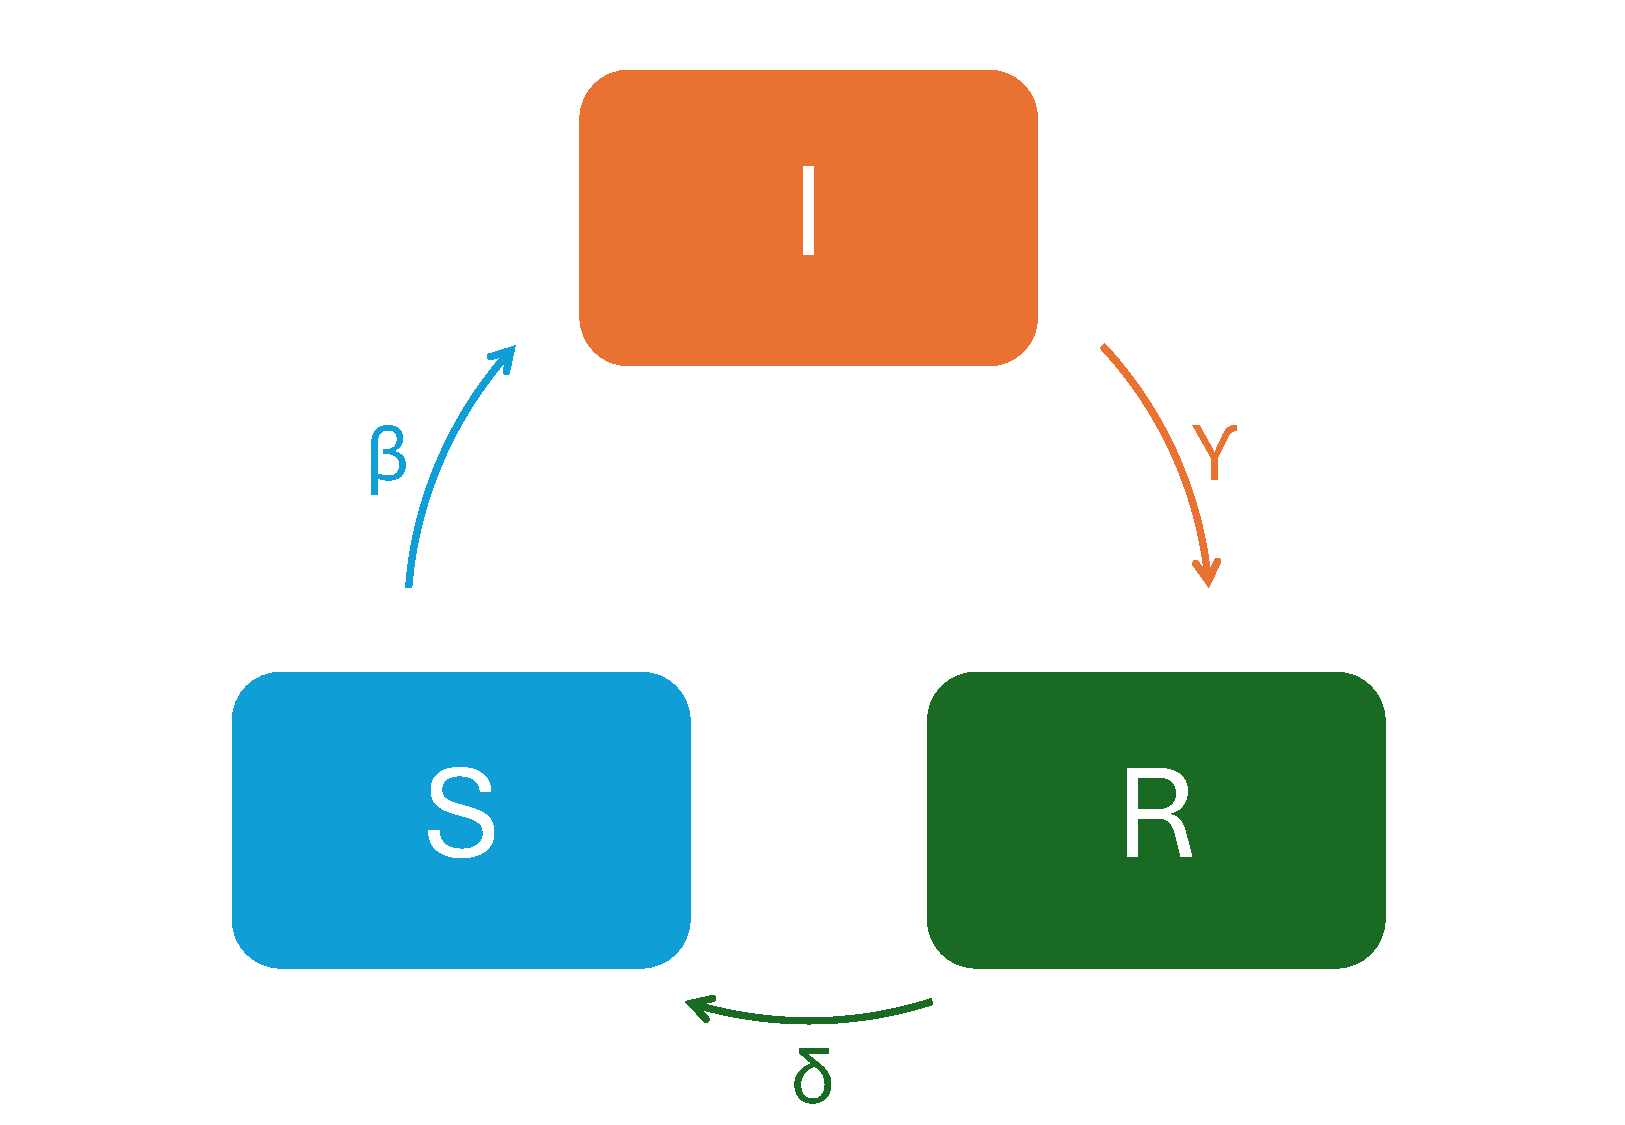
\includegraphics[width=0.65\linewidth]{0_introduction/images_introduction/SIRS_figure_compartmental}
	\caption[SIRS example]{An example of the graph structure of a mean field SIRS model. There are three compartments and the flow rate between them is ruled by the coefficients $\beta$, $\gamma$ and $\delta$.}
	\label{fig:sirsfigurecompartmental}
\end{figure}


\subsubsection{SIR model}
\label{subsec:SIR}
The foundational model for studying epidemics mathematically is the SI model. In this model, the population is divided into two compartments: Susceptible $(S)$ and Infected $(I)$. Individuals transition from being susceptible to infected, but there is no recovery, meaning once infected, individuals remain infectious indefinitely.

An extension of this is the SIR model, which adds a third compartment, Recovered $(R)$. This additional compartment represents individuals who have either gained immunity or have died, removing them from the cycle of infection. After spending a certain period in the infected state, individuals transition to the recovered state, making them no longer susceptible to the disease.
Here the population or density of individuals is divided into three groups: Susceptible, Infectious, and Recovered. At time $t$ the three groups are identified with the symbols: $S(t)$, $I(t)$, and $R(t)$. 
The symbols used to indicate the density of each group are $s$, $i$, and $r$, while the capital letters are used to specify both the name of the groups or the absolute number of participants in each one. 

The SIR model, which will be described in the following sections, is built upon several foundational assumptions that shape the mathematical framework. These guiding principles are introduced here and will be encountered throughout the model's developed in this thesis. Understanding how the model operates is crucial, as these assumptions are essential to the structure and behavior of the model itself.
\subsubsection{Neglected demographic influence}
The total population size, represented by the letter NN, is the sum of individuals in the three compartments (e.g., Susceptible, Infected, and Recovered). It is often assumed to remain constant during the course of an epidemic. This assumption is based on the idea that epidemics typically last much shorter than the average human lifespan, making the effects of births and deaths negligible.
In more complex models, where demographic effects are considered, such as in models of longer-lasting epidemics, the population size can still be assumed constant by balancing the number of births (modeled as an influx into the Susceptible compartment) with the number of deaths (modeled as an outflux). This approach assumes that births and deaths occur at approximately the same rate, keeping the total population size stable over time. The result of this assumption implies that:
\begin{itemize}
	\item Population density compartments sum up to one.
\end{itemize}
\[s(t) + i(t) + r(t)= 1 \]
\begin{itemize}
	\item The sum of the derived functions w.r.t. time is equal to zero.
\end{itemize}
 \[\dot{s}(t)+ \dot{i}(t) + \dot{r}(t)= 0\]

\subsubsection{Recover transition} 
The first fundamental dynamic process of the model assumes that the infected compartment decreases in size independently of the model's history, with a rate of decrease proportional solely to the current number of infected individuals. This gives the following relation:
\[\frac{d i}{dt} = - \gamma i, \qquad i(0) = i_0., \]
which models a continuous process. Specifically, it assumes that individuals transition from the infectious state to the recovered state at a constant rate, denoted by $\gamma$. The physiological meaning of this parameter is that it represents the inverse of the infection's duration, meaning the average infection lasts $1/\gamma$ days. Thus, $\gamma$ is the recovery rate, reflecting the speed at which the population recovers from the disease.
 
In this model the disease reproduces through horizontal incidence, and so the contagion is modeled as due to random contact that happens in a homogeneosuly mixed population.
\subsubsection{Person-to-person disease transmission}
The model for this quantity is expressed in fractional terms, assuming a population composed of susceptible and infected individuals. Each infectious individual encounters a fraction cc of the population per day. If all encounters are equally likely, a fraction $s$ of these encounters will be with susceptibles. Therefore, each infectious individual has $c\cdot s$ encounters with susceptibles. The probability that an encounter leads to transmission is $p$, meaning the average number of transmissions per day is $p \cdot c \cdot s$. Considering the fraction of infected individuals, and combining $p$ and $c$ into a single parameter, the transmission rate becomes:
\[\text{transmission rate} = \beta s i.\]
Here, $\beta$ represents the transmission coefficient.


\subsubsection{Immunity}
In this initial model, once individuals recover from the disease, there are no further transitions. This can be due to two possible scenarios:
\begin{itemize}
	\item Lifelong immunity acquired after recovery.
	\item Death of infected individuals, if demographics are considered.
\end{itemize}
Both cases assume that once the illness period ends, the disease can no longer be transmitted.
If immunity acquired from an infection wanes after a certain period, individuals can become susceptible again, leading to an SIRS model.

\subsubsection{Threshold value}
Although the SIR model is simple, it plays a fundamental role in predicting a key aspect of epidemics: the threshold value, a concept first introduced by Kermack and McKendrick in their pioneering work \cite{kermack1927}. They showed that in a fully susceptible population, an epidemic will only start if the basic reproduction number $R_0$ is greater than $1$, marking the birth of the term "threshold value" in epidemiology.

Over the years, the dynamics of this system have been extensively studied and analyzed \cite{Breda_2012, akinboro2014numerical, Jard_n_Kojakhmetov_2021, Ledder_2023, Okabe_2020, Prodanov_2022, Xu_2014, Turkyilmazoglu_2021}. The threshold effect highlights two distinct scenarios:
\begin{itemize}
	\item \textbf{Free Disease Equilibrium $(R_0 < 1)$:} When $R_0$ is less than one, the disease does not spread within the population. Although infected individuals make contact with susceptibles, the rate of disease transmission is slower than the recovery rate. Mathematically, this means $\beta / \gamma < 1$, or $\beta < \gamma$, where $\beta$ represents the transmission rate and $\gamma$ the recovery rate. Consequently, the healing process is faster than the spread of infection, and the number of infected individuals quickly drops to zero. The majority of the population remains susceptible, and this state is globally asymptotically stable, as demonstrated by \cite{Hernandez_Vargas_2022}.
	\item \textbf{Epidemic spread $(R_0 > 1)$:}     When the threshold is greater than one, the number of infected individuals grows until it reaches a peak and then declines toward zero. The peak number of infected people, as well as the final number of susceptibles, can be calculated using the system's initial conditions and the values of $\beta$ and $\gamma$, as described by \cite{Hethcote_2000}. This scenario illustrates how a highly aggressive infection can spread widely within a population. If no countermeasures are taken, it can lead to significant social and economic consequences.
\end{itemize}
	Thus, even with its simplicity, the SIR model provides critical insights into the potential severity of an epidemic and highlights the importance of timely interventions to prevent widespread harm.
\subsubsection{Derivation of I evolution and SIR differential equations presentation}
After having theoretically presented the model, it is now explained one method to derive the mathematical form of the infection compartment evolution. 
The set of differential equations that  describe the dynamic of infection is the following:
\begin{equation}
	\begin{cases}
		dS(t) / dt = -\beta S(t) I(t)\\
		dI(t) / dt = \beta S(t) I(t) - \gamma I(t)\\
		dR(t) / dt =  \gamma I(t)
	\end{cases}
\end{equation}
Here $X(t)$ is indicated as the population at time $t$ in the X compartment. Remember that the assumption of constant population size is also done, so $S(t)+I(t)+R(t) = N$ holds.

The number of infected, with an interval  $\Delta t$, that in a base case can coincide with one day, is given by the equation:
\begin{equation}
	I(t+\Delta t) = I(t) + [\beta S(t)I(t)/N - \gamma I(t)]\Delta t
\end{equation}

If the value of N is large, the variables can be considered as continuous, and imposing a time interval close to zero it becomes:

\begin{equation}
	\frac{d I(t)}{dt} = \lim_{\Delta t \rightarrow  0} \frac{I(t+\Delta t)-I(t)}{\Delta t} = \beta S(t) I(t)- \gamma I(t)
\end{equation}

Consider now the initial state of the system. At the beginning of the disease, considering that there are few infected, the majority of the population is in the susceptible groups, so $S(0) \approx N$. Furthermore, during the initial days of contagion diffusion, this quantity remains stable. Considering this approximation, we have 
\begin{equation}
	\frac{d I(t)}{dt} = (\beta S(0)-\gamma)I(t),
\end{equation} 
which gives now a differential equation with only a variable, $I(t)$, that has a well-known solution:

\begin{equation}
	I(t) = I(0) \exp ^{(\beta S(0)- \gamma)t}
	\label{eqn:sol_I}
\end{equation}



From the analytic solution of the infectious dynamic equation in \ref{eqn:sol_I}, we can see what happens at the beginning of an epidemic.  If the exponential argument has a positive sign it is observed an exponential increase in the number of infected. While, in the opposite case, infected people tend to zero. 
The value $\frac{ \beta}{\gamma} S(0) = 1$ is defined as the epidemic threshold. In the initial phase of the epidemic the relation $\frac{ \beta}{\gamma} S(0) = \frac{ \beta}{\gamma} N $  holds. 
This quantity, normalized, is called the basic reproductive rate, and indicated with the symbol $R_0$.

It measures the intensity of the contagion or the number of secondary infections a sick person can generate. Analysing the equation of susceptibles, with this model we see that it is always decreasing. In the SIR model, if the condition to start the epidemic is satisfied after an increase in the number of Infected, there is a point at which $\frac { \beta}{\gamma} S(0)$ becomes less than one. It is when this happens that the peak of the $I(t)$ curve is reached. Then, the disease begins its falling phase. It is the natural behavior of an epidemic.

\begin{figure}[h]
	\centering
	\subfloat[][\emph{}]
	{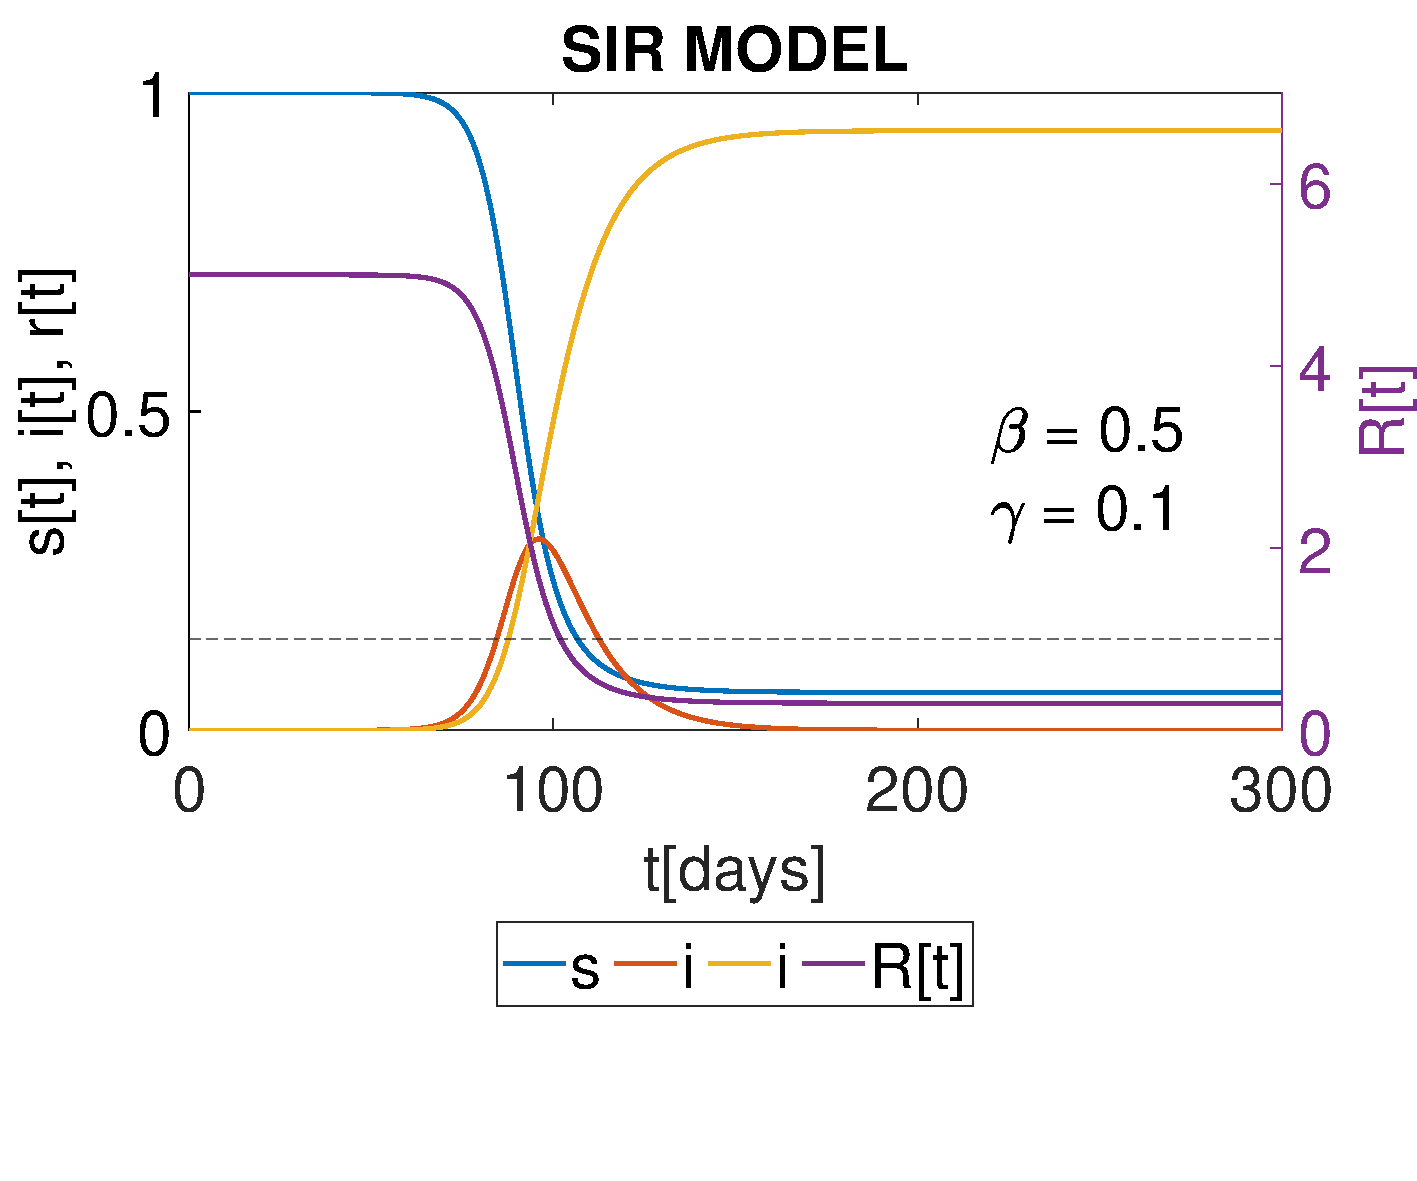
\includegraphics[width=0.48\linewidth]{0_introduction/images_introduction/sir_con_rt}} \quad
	\subfloat[][\emph{}]
	{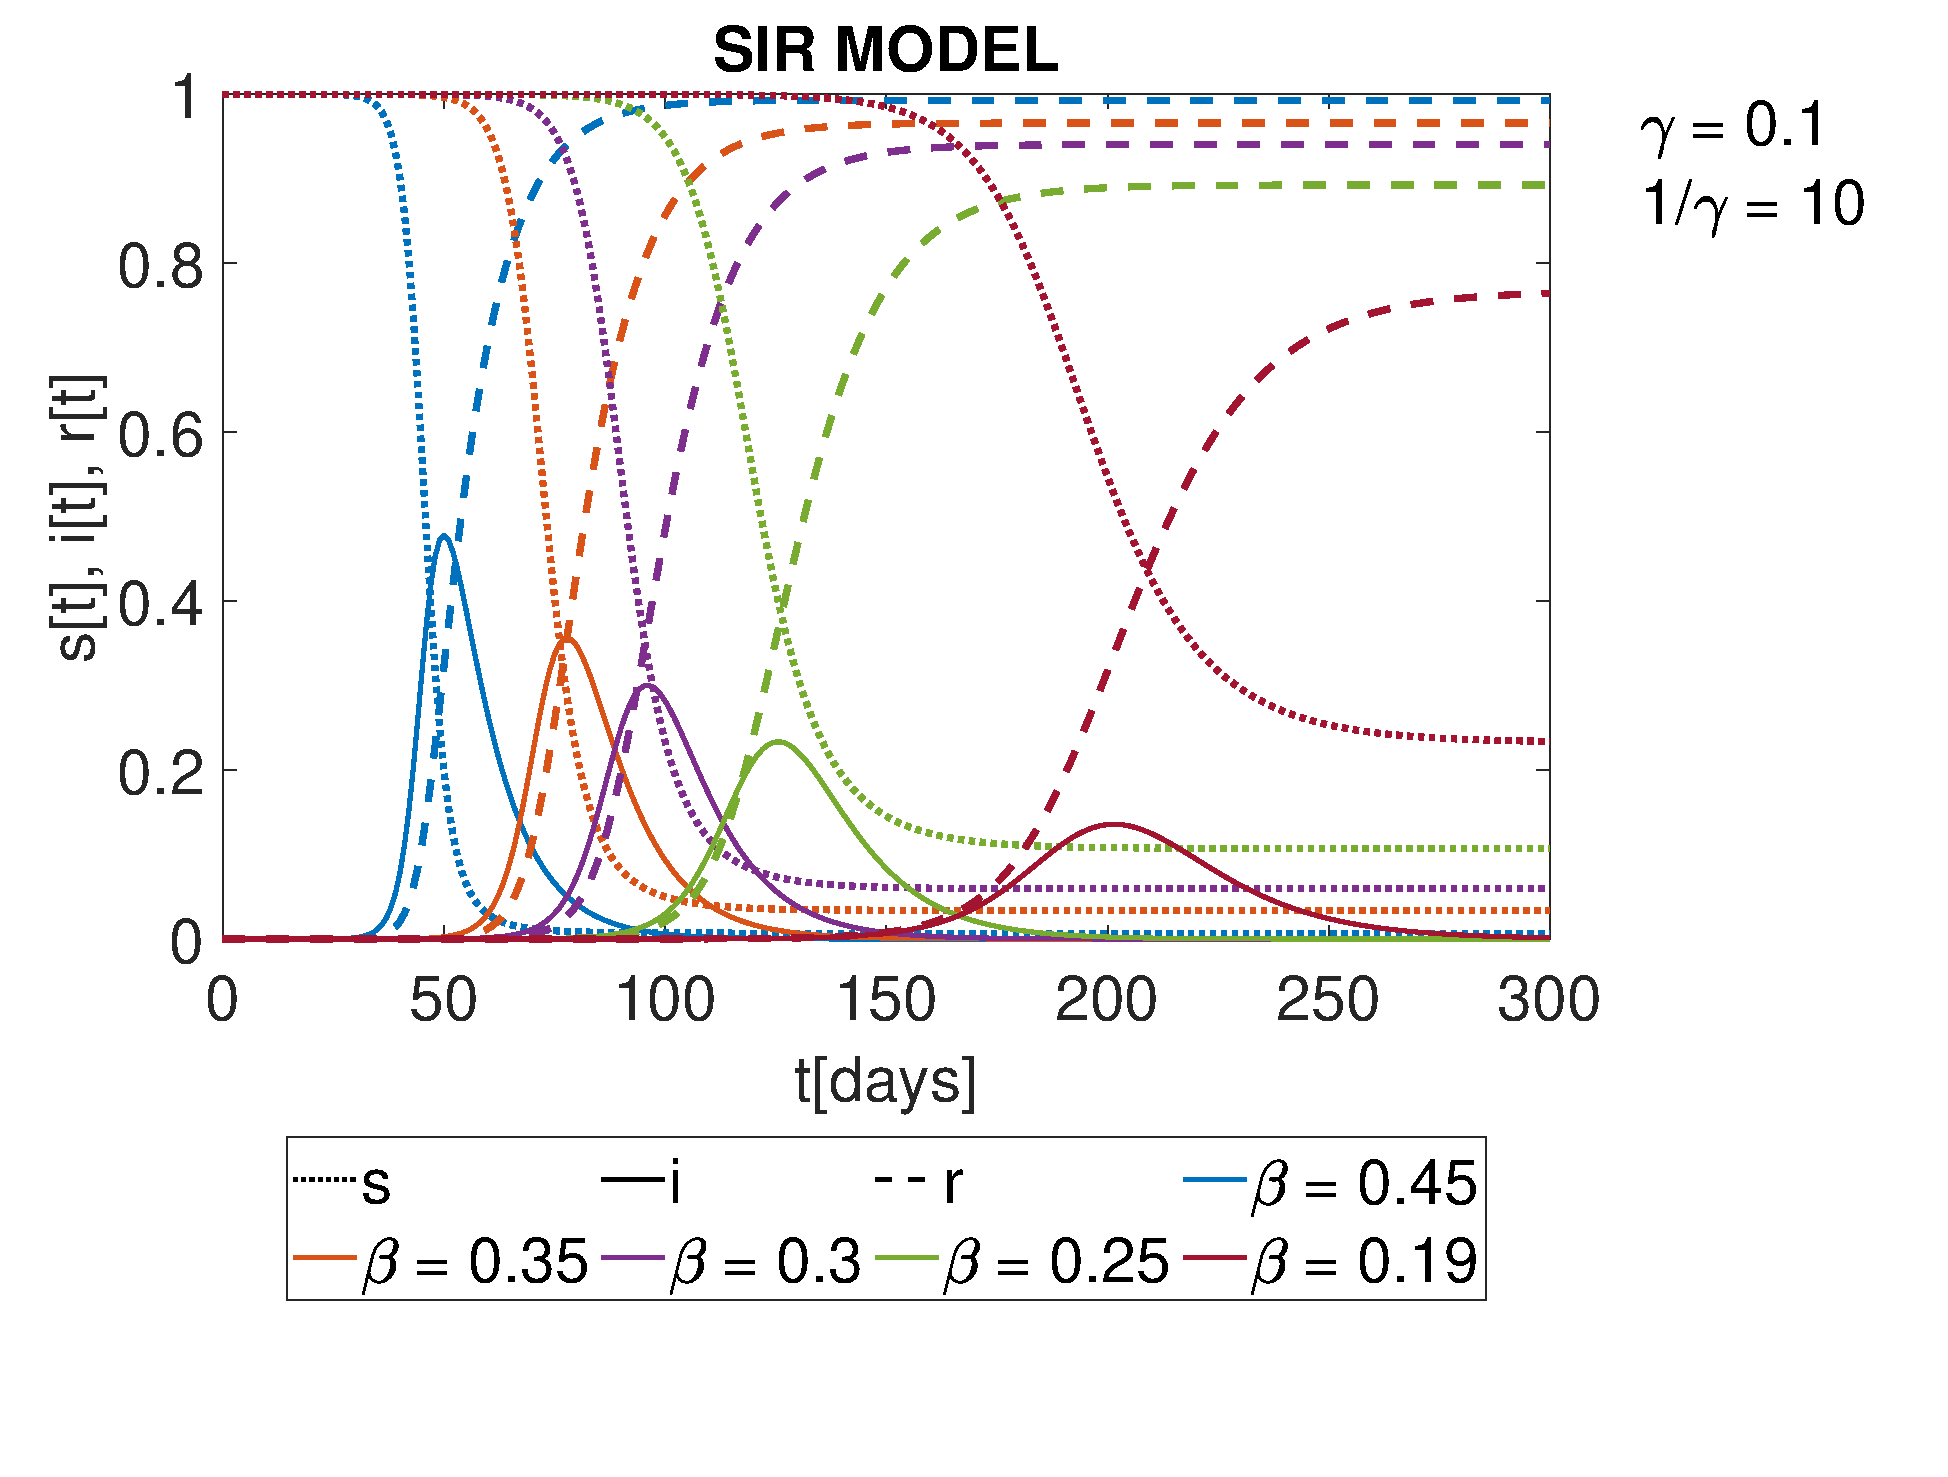
\includegraphics[width=0.48\linewidth]{0_introduction/images_introduction/sir_multipli_beta}} \\
	\caption[SIR dynamic example]{SIR system numerical solutions. Figure a) shows the evolution of compartments in the case of an epidemic. The violet dotted line represents the time-dependent $R_0(t)$. It can be seen that when this parameter is equal to $1$, the number of infected reaches its maximum value. In b) are presented different evolutions of the disease varying only the $\beta$ coefficient. The smaller its value the flattened and the more delayed the infectious curve is.}
	\label{fig:sir_example}
\end{figure}
Other two interesting quantities to consider when a new disease appears are the rate of increase of the infectious and the final size of remaining susceptible at the end of the epidemic. There is a large difference when a population suffers from an epidemic if this ends rapidly because a lot of people get sick or if this number can be controlled, and the infectious curve is flatter. A strategy to flatten the curve can reduce the contact between susceptibles, actuating social distancing or avoiding contact with infected, implementing quarantine measures. These are two simple examples of actions that reduce the value of $\beta$. Another countermeasure is represented by vaccination. Its immediate effect on the epidemic is to remove susceptibles people, so the disease can afflict only a small group and be quickly extinguished. 

\subsubsection{Stochastic models} 	
This is a group of models deriving by the mean-field, but using a different mathematical approach.
In this typology, the transition from one state to another is determined using a function of probability.  Conceptually are derived using the same framework used with ODE models. They are useful when the disease to study has a lower number of infected or if there is a connection between the epidemic outcome and changes in individual dynamics. This is called demographic variability, and it concerns changes in transmission, births, recovery, or deaths within the population. Using stochastic models with Monte Carlo simulations can be useful to investigate epidemic models on networks \cite{Allen2017}. 
The two most important types of models using this approach consider the time variable as continuous, $t \in [0, \infty) $and then the state variable is either discrete (Continuous-Time Markov-Chain) or continuous (Stochastic Differential Equations).
Referring to the SIR model to make a simple example here the S and I compartments are modeled as random variables. The probability of individuals changing groups depends on infection and recovery, the possible events that can occur. It is called transition probability. 
In a Markov chain approach the transition probability is discretized, and there is no dependence on the history of the epidemic to know how it will evolve at time $t + \Delta t$. It is necessary to know only the current state of the process at time $t$. 
In the Stochastic differential equation, the random variables are continuous. 

\subsection{Networked models}
\cite{Newman2002}, \cite{VanMieghem2009}, 
The evolution of a disease is considered over complex and realistic networks. The focus of this type of model is to understand how the network structure influences the epidemic by observing parameters such as the rate of spread.

In this framework, the nodes of the graph represent individuals (with all the properties that the modeler deems relevant for the study), while the edges represent interactions between people. Nodes can also represent subgroups of people, and using weights on edges makes it possible to characterize the strength of these interactions.

Only if this class of model is highly capable of realistically reconstructing a real network can it be a reliable instrument, and achieving this requires very complex work.
\subsection{Agent-based models}

VEDI E AGGIUNGI ANCHE \cite{Tizzoni2014}

DA WIKI INTEGRA: "An agent-based model (ABM) is a computational model for simulating the actions and interactions of autonomous agents (both individual or collective entities such as organizations or groups) in order to understand the behavior of a system and what governs its outcomes."

Agent-based models are an alternative technique used to represent disease evolution. This approach is implemented based on the observation of spontaneous connections made by individuals. 
An advantage of this type of model is that it offers a very intuitive approach to epidemic modeling. Using an individual perspective guarantees an immediate interpretation of the model. A precise agent-based model can provide a greater understanding of the illness under consideration and direct information about countermeasures to implement to stop or mitigate its spread. However, to be powerful and capable of performing good analyses and predictions, a lot of information must be integrated into the model. 
\begin{figure}
	\centering
	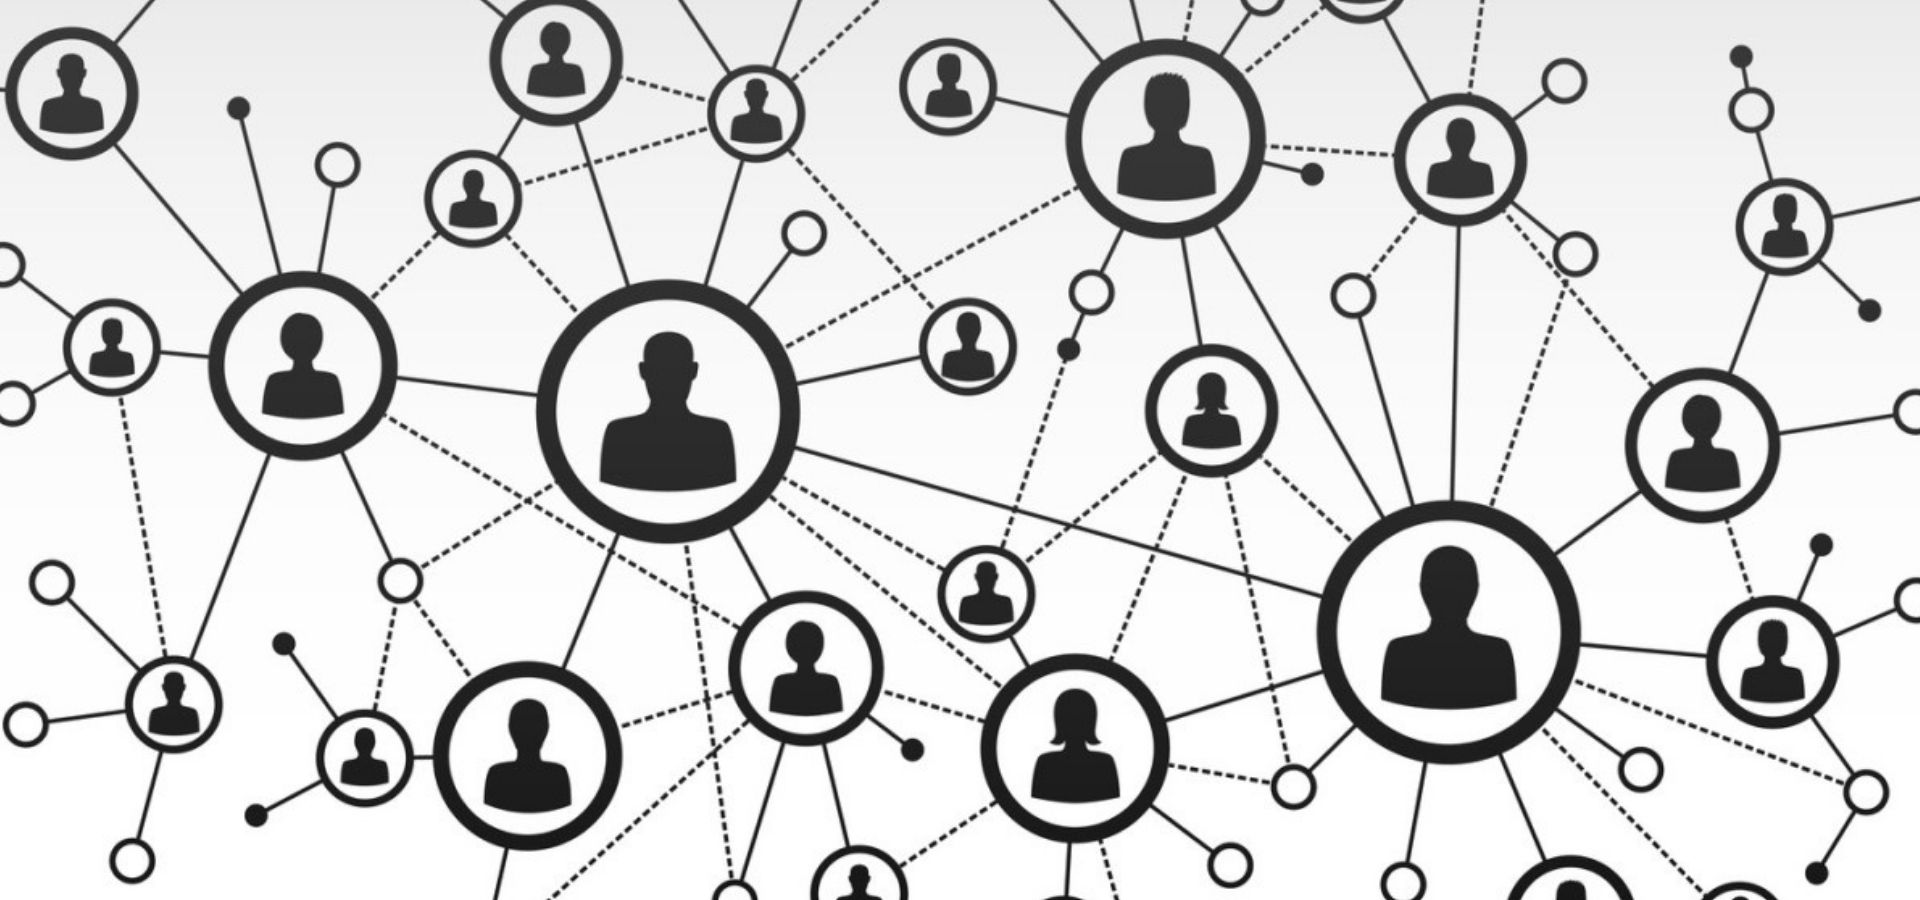
\includegraphics[width=0.5\linewidth]{0_introduction/images_introduction/agent_based}
	\caption[Agent based network representation]{Agent based network representation}
	\label{fig:agentbased}
\end{figure}

%%

An example of a possible mathematical implementation of this class of models is now briefly presented. One possible technique to describe peer-to-peer contact in a graph structure is realized through a probabilistic framework. Here, assuming a total of $n$ agents in the model, spread processes can be described as a function of probability. Using Markov processes, each agent has a certain probability of transitioning from one state of the disease to another. To calculate the value of these probabilities, both the information derived from the network structure and parameters related to the disease, such as infectivity and recovery rates, are used. In this way, a stochastic evolution model of the processes is developed.

Considering an SIS model described with a Markov process: it has a dimension of $2^n$, while implementing an SIRS model requires a dimension of $3^n$. Because the size of models developed in this manner becomes rapidly enormous, a mean-field approximation is employed. It is based on the assumptions of a network composed of a sufficiently large number of agents and on the independence of these nodes. With this technique, by taking expectations, the transition rates of individuals are approximated. Using these approximations, the boundary values of the agent's probability of infection can be determined at each time step \cite{Hernandez_Vargas_2022}.

\subsection{Multilayer systems and networks} 

AGGIUNGI ANCHE \cite{Wang_2019} \cite{Krickel_2023}

The complex dynamic of interactions existing in the real world, develops in multiple patterns, with complicated relationships. This connection can change over time, and using the theory of multilayer systems it can improve the comprehension of such complexity. Additional information can be added to the model, for example, different types of interactions, like physical contact or information sharing, time dependency coefficients, or reliance between different parameters in nature, creating cause-effect relationships. 
It is a more recent development of the research, the traditional network theory was revisited, to create a framework that can include multiple networks, that evolve and influence each other \cite{DeDomenico2016} and can be helpful to manipulate complex systems like human relationships. Some interesting results obtained are the possibility that the onset of one disease can depend on the onset of the other one. There can be regimes in which the criticality of the two dynamics is interdependent and others in which the critical effect is only one-directional \cite{DeDomenico2016}. 
One possible way to develop models with this structure is to imagine that each layer represents a different type of interaction. An epidemiological example is a layer in which the physical contact between people is simulated and another represents social structure, the network of relations that every person has. This instrument provides a natural representation of coupled structure and dynamical processes. It has been presented in multiple works in the past years, for example in CITA. 
The dynamic realized in multiple systems can be single or coupled. In the first, there is a top layer with its dynamic evolution running on top of a multilayer network. The coupled structure instead is the one in which the phenomena described in each layer evolve with the influence of what is happening in the other. 
Multilayer networks have multiple dimensions of connectivity, called "aspects" and they have to be considered simultaneously. 
They can also be considered with two different mathematical structures. 
\begin{figure}[]
	\centering
	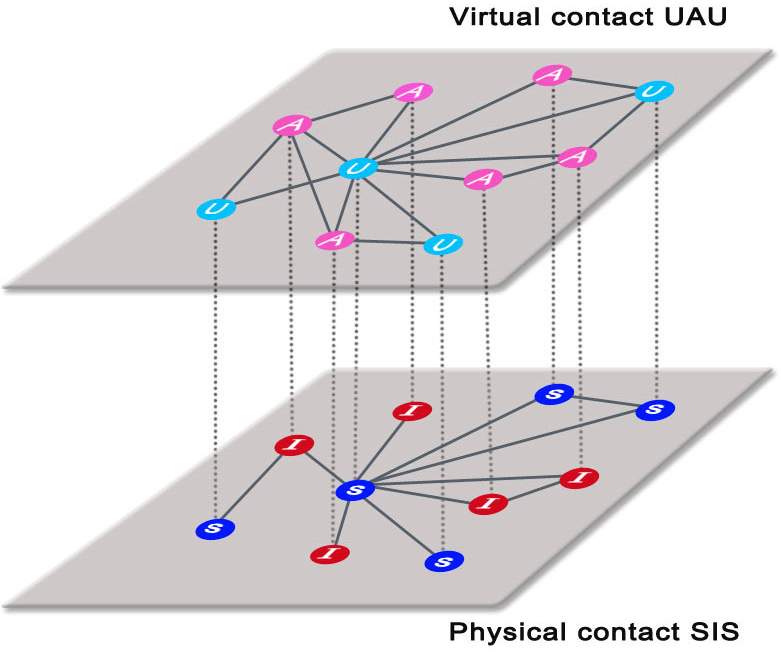
\includegraphics[width=0.6\linewidth]{0_introduction/images_introduction/multi_layer}
	\caption[Multi-layer network]{Representation of a multiplex structure. The figure is taken by the work of \cite{Granell2013} and shows the network implemented in their model. There is an awareness and an epidemic layer. In this case, the node connected with the interlayer connection represents the same individual.}
	\label{fig:multilayer}
\end{figure}

The first uses the same set of compartmental structure and mean-field models presented in the section before \ref{subsec:mean_field}. Here, from a mathematical point of view, there is no such difference in the manipulation and analysis of the system. The distinction relies on the meaning of the compartments and parameters created and on the dependence of the coefficients, which can be time and state-dependent.

The second option considers an agent-based structure. Here, considering a graph structure, composed of nodes and links between them, it is possible to classify three types of edges:
\begin{itemize}
	\item intra-layer edges, the connection of nodes on the same layer.
	\item inter-layer edges, the connection between a replica of the same node, but lying on a different layer of the structure;
	\item inter-layer edges, but coupling nodes representing distinct entities. 
\end{itemize}

 
%%%%%%%%%%%%%%%%%%%%%%%%%%%%%%%%%%%%%%%%%%%%%%%%%%%%%%%%%%%%%%%%%%%%
\chapter{Review of epidemiological behavioural and opinion models in literature}
\label{ch:literature_review}
%NUOVO TESTO
The scientific community's interest in epi-behavior models has existed for several years. Initially, as noted by \cite{Bauch_2012_overview}, the behavioral aspect of epidemiology was not given significant attention. Its development has been a gradual process, resulting from years of evolution in research.

In fact, in the initial works \cite{kermack1927}, the focus of scientists was primarily on presenting the evolution of diseases. The resulting models did not account for the effect of behavior; the population was considered homogeneously mixed, leading to random contact between susceptibles and infectives \cite{Hernandez_Vargas_2022, Mata2021}. 
It was only later, as epidemiological models proved to be effective and reliable in describing and predicting disease spread, that interest among policymakers grew. Tools capable of integrating real data with epidemiological models emerged, aiding decision-making on matters such as the duration of school closures or travel restrictions, as described in \cite{Bauch_2012_overview}.

Furthermore, new categories of models have emerged, such as agent-based models, networked models, and multi-layer/multi-system models. Despite their differing approaches, they aim to integrate various population characteristics, for example contact structure, age distribution, and movement patterns, to address the limitations of the original homogeneity assumption \cite{brauer2012mathematical}.
This focus on societal composition and behavior naturally stems from the desire to use modeling tools as a reference for decision-making in safety and health. 
One possible approach is to incorporate changes in the structure of models that describe aspects of behavior or population composition.

In these models, the behavior of the population is implicitly considered by integrating time-variable parameters that capture changes in societal behavior. This approach represents the classical modeling technique used in the formulation of epidemiological models. Examples of studies that uses this methodology for analyzing COVID-19 include \cite{Giordano_2020, Dehning_2020, Proverbio_2021}.

Although models developed in this way have proven to be powerful tools for generating insights about disease dynamics and providing recommendations to policymakers, they fall short in their ability to accurately reconstruct how populations behave during an epidemic outbreak. The desire to explore this aspect and develop a framework capable of simultaneously simulating both behavior and disease diffusion—where each mutually influences the other—has driven the development of a specific research field dedicated to behavioral epidemics.

But how can behavior be integrated into pre-existing epidemiological theory? To better address this question, we follow the classification proposed in \cite{Funk_2010}, which offers a possible subdivision of behavioral literature based on the different approaches that most articles focus on. Three major categories emerge:
\begin{itemize}
	\item The source of information used to make decisions;
	\item The type of information used to make decisions;
	\item The effect of behavioral change on the dynamic described by  the model. 
\end{itemize}

\section{Information's sources}
When analyzing the source of information, there is a clear distinction between works \cite{Vogiatzis2010} that assume governments and populations base their decisions on precise data, such as the number of infected individuals (prevalence) \cite{Collinson2014, Tyson_2020}, and those that consider more informal sources, such as conversations between people, public opinion, or media \cite{Bulai2023, Sontag2022}. These media sources include both traditional outlets like television and newspapers, as well as newer platforms like social networks.
This distinction highlights the diversity in how behavioral factors are integrated into models, reflecting the varying degrees of reliability and influence these sources have on decision-making processes during an epidemic.


Regarding information quality and the negative effect of misinformation spreading within the population, an example is the fear of vaccination \cite{Kahan_2013}. Several works analyze its effects to on the spread of infection \cite{Bauch_2012_game, Epstein_2021}.
An example of how this phenomenon can arise is the story of an article originally published by a prestigious source. Even though the thesis presented in this work was later proven wrong by the scientific community \cite{wakefield1998retracted}, the negative impact in terms of spreading fear about vaccines has persisted and, in many cases, has become deeply ingrained. In this specific case, it caused a decrease in herd immunity and a resurgence of measles \cite{Bauch_2012_overview}.

\section{Classification of different types of information}
After introducing the impact that information quality may have, another interesting aspect is related to the different types of information used in model development. Some articles focus on the effect of media on behavior \cite{Collinson2014, Misra_2011}, while others consider peer-to-peer conversations, information exchange, and beliefs among individuals \cite{Tyson_2020}. These are completely different approaches, even though they aim to achieve the same effect: simulating the evolution of people's opinions and behavior. Using media involves hypothesizing that the population is influenced by a few "central" information nodes, so the same news, data, or future predictions are shared with everyone. In contrast, models that use personal information exchanges can depict a scenario where many different ideas about the disease situation circulate simultaneously.
Another concept used in models that simulate a sort of "collective consciousness" is referred to as "awareness" \cite{Funk2009}. To model how awareness spreads in the population, it is often treated like a disease \cite{Silva2019, Granell2013, Granell_2014, Kabir_2019, Zuo_2021, Wang_2019}. Although there are many differences between these two, the main idea is that theories and concepts about a certain topic can spread among people, which can be considered at a higher level as a unified opinion. For example, there may be many different personal positions on how to respond to a health emergency like COVID-19, but it is possible to abstract the various opinions and reconstruct what the majority of people, or macro-groups, ultimately feel. They may either be more cooperative and in favor of following guidelines issued by authorities, or more focused on their well-being and inclined to act independently.
This process can be related to opinion formation studies, which aim to understand how people build their ideas \cite{Devia_2023, Devia2022} and also analyze the possible formation of opinion distributions, such as perfect consensus, consensus, polarization, clustering, or dissension.

\section{How integrate behavior in epidemiology}
While the type and source of information are crucial for understanding the basic framework and synthesizing key concepts of models that consider population behavior, the final criterion used to categorize works related to epidemiological behavior is how the influence of people's behavior on the model is integrated. This aspect is one of the most interesting and was a key focus of the literature reviewed for this thesis, as it plays a significant role in comparing and selecting relevant works for this research.

There are various ways to describe behavior in response to an epidemic and integrate this aspect into epidemic models \cite{Wang_2019, Bedson2021, Wang_2015_review}.

The first approach involves observing and simulating how connected individuals' states are linked to specific behaviors and how this influences the epidemic. This category includes agent-based models. Additionally, the reverse relationship, where disease spread alters individual behavior, has also been considered, as discussed in \cite{Granell_2014}.

There is also a broad class of mean-field models that explicitly consider the effects of behavior. In these cases, time-varying or state-varying parameters are used, resulting in a non-linear system of equations where the parameters are not constant but change based on information such as disease prevalence. Refer to paragraph \ref{subsec:homogeneous} for further details on this topic.

Another possibility involves modifying the structure or connections in the network used to simulate disease evolution \cite{Peng2021}. In network-based models, data extracted from social network structures \cite{Carballosa_2021} or small-world models \cite{Turker_2023} are often used to simulate connections between people more realistically.

In the following paragraphs, several articles are presented using this classification to simplify their categorization. Each article is then discussed in more detail, highlighting its original contribution.

\subsection{Models in which change the individual' state}
\label{subsec:individual_state}
\subsubsection{Multiple network simulated with Markovian process}
The first presented work is done in \cite{Granell_2014}. Here, a multiplex model is implemented with two different connectivity layers: the physical layer, in which spreads the disease, and the virtual contacts layer, where awareness diffuses. The article then uses the Microscopic Markov Chain approach to simulate the interaction resulting from the coupling of the two layers. Interestingly, they observe the existence of a metacritical point for the onset of the epidemic, which depends on awareness dynamic and topology of the virtual network. There is, in fact, a parameter related to the ability to influence through communication and it is observed that it impacts the onset of the epidemic only when it exceeds a certain threshold.
A subsequent work of the same authors \cite{Granell2013}, considers also the effect of a global communication agent. In this case, the metacritical point disappears. 
\begin{figure}[h]
	\centering
	\subfloat[][\emph{}]
	{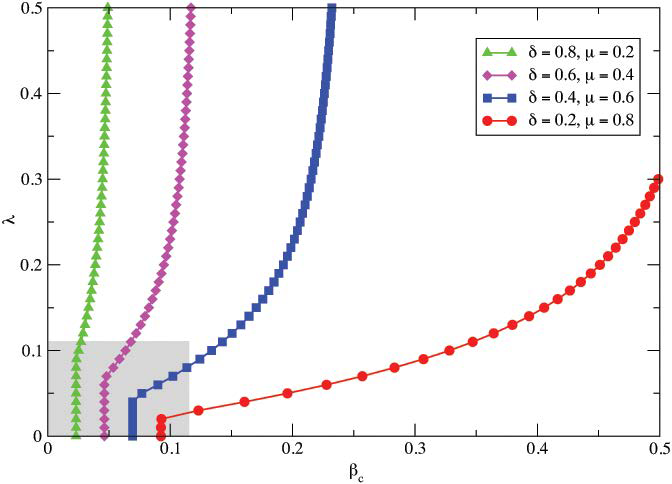
\includegraphics[width=0.47\linewidth]{0_introduction/images_review/metacritical_point_granell_2013}} \quad
	\subfloat[][\emph{}]
	{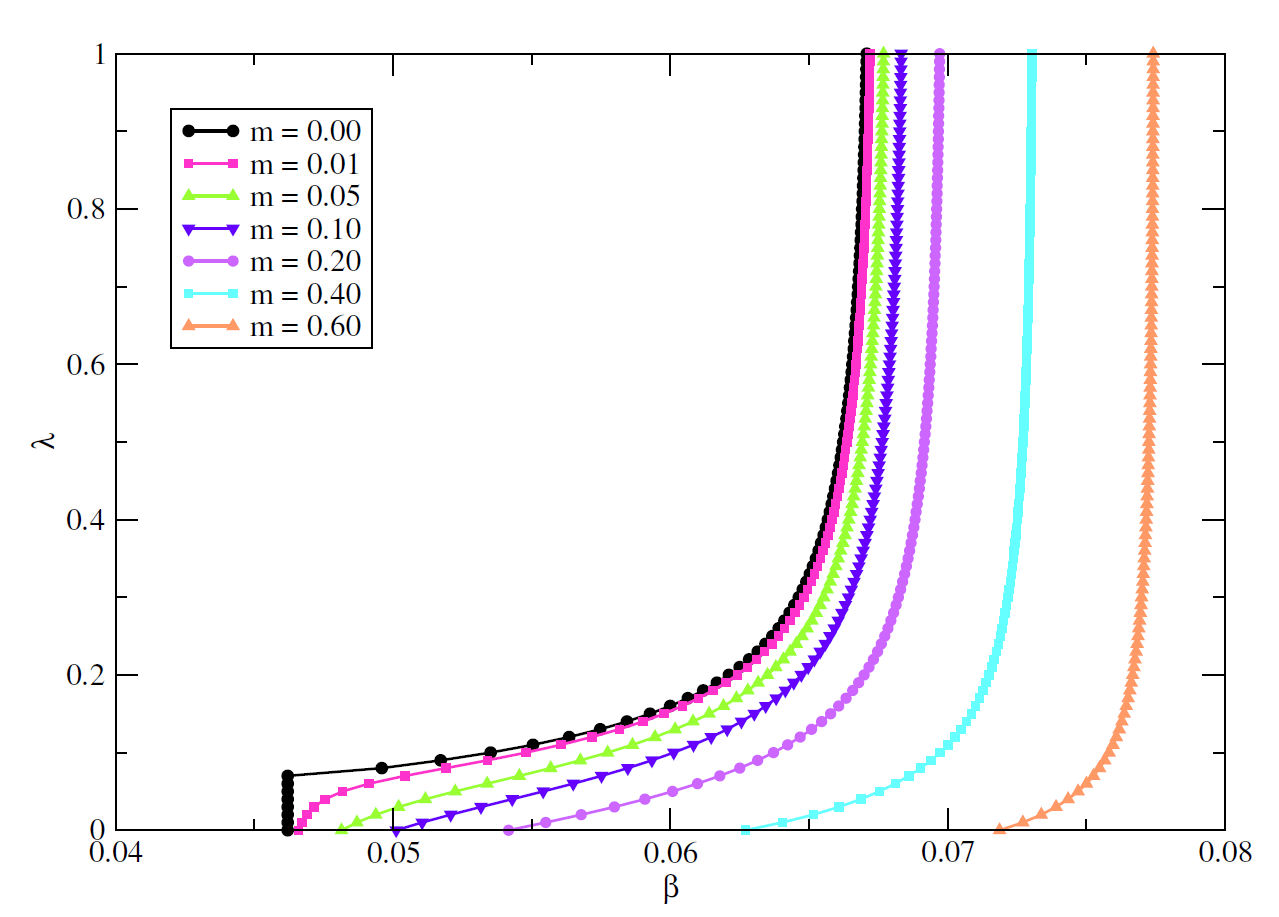
\includegraphics[width=0.49\linewidth]{0_introduction/images_review/metacritical_point_granell_2014}} \\
	\caption[Metacritical effect]{Effect of awareness communication on the onset of an epidemic. Pictures taken from \cite{Granell2013, Granell_2014}. In (a), the metacritical region is highlighted, showing that below a certain influence value $\lambda$, awareness has no significant impact on the epidemic dynamics. Conversely, in (b), the influence of a media parameter $m$, representing a global communication agent, ensures that the epidemic is always affected by the awareness layer.}
	\label{fig:sir_example2}
\end{figure}


In the article by \cite{Sahneh2013}, there is a complete description of the stochastic process at the agent level, which is useful for understanding how agent interactions are modeled across different layers using a Markovian approach. Other works using this method include \cite{Silva2019, Frieswijk_2022, Peng2021, Zuo_2021}. Except for \cite{Frieswijk_2022}, a similar double-layer structure, composed of an SIR model coupled with a UAU process, is presented in the other articles. To simulate the evolution of the complex structure resulting from the coupling of the two models, they build transition trees for all possible state changes and their respective transition probabilities. An example of both can be seen in figure \ref{fig:sir_example3}.  

\begin{figure}[h]
	\centering
	\subfloat[][\emph{}]
	{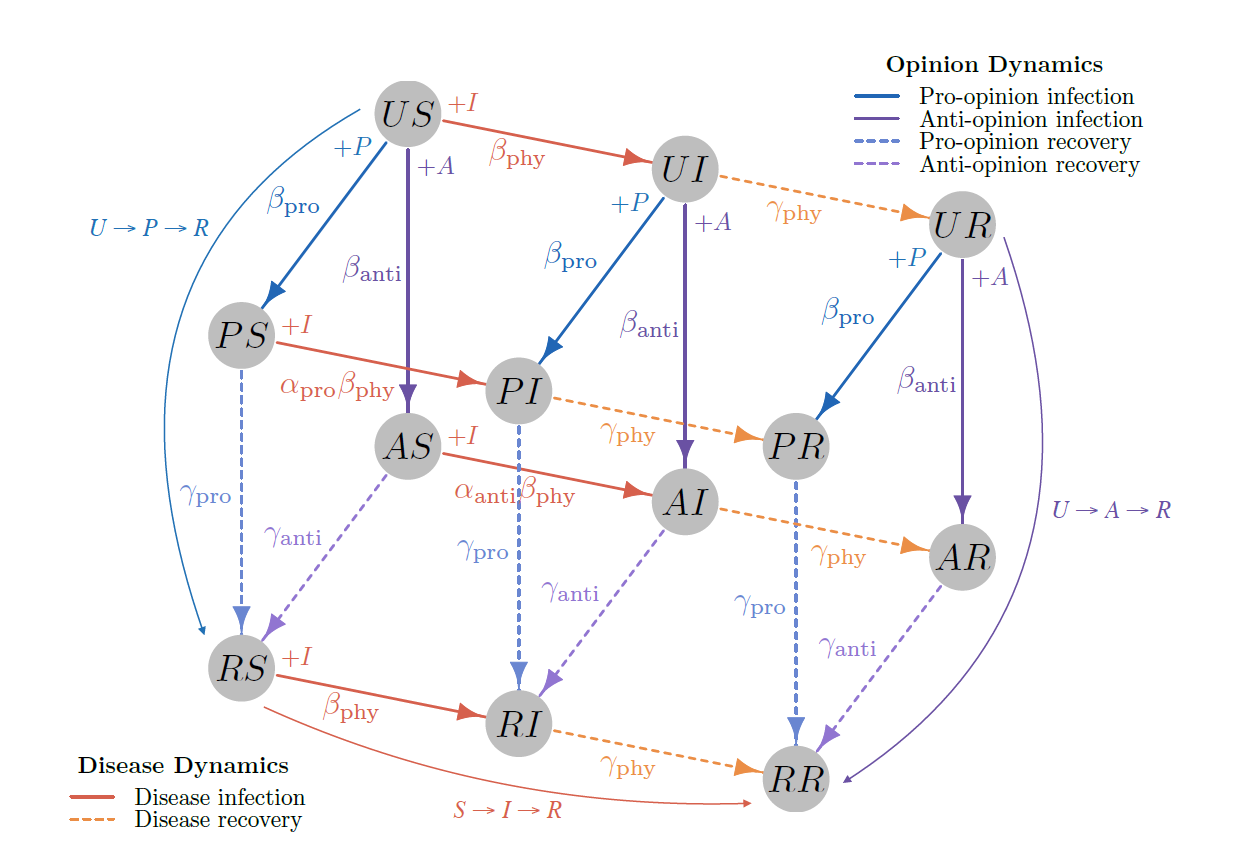
\includegraphics[width=0.63\linewidth]{0_introduction/images_review/peng_2021_bertozzi_coupled_structure}} \quad
	\subfloat[][\emph{}]
	{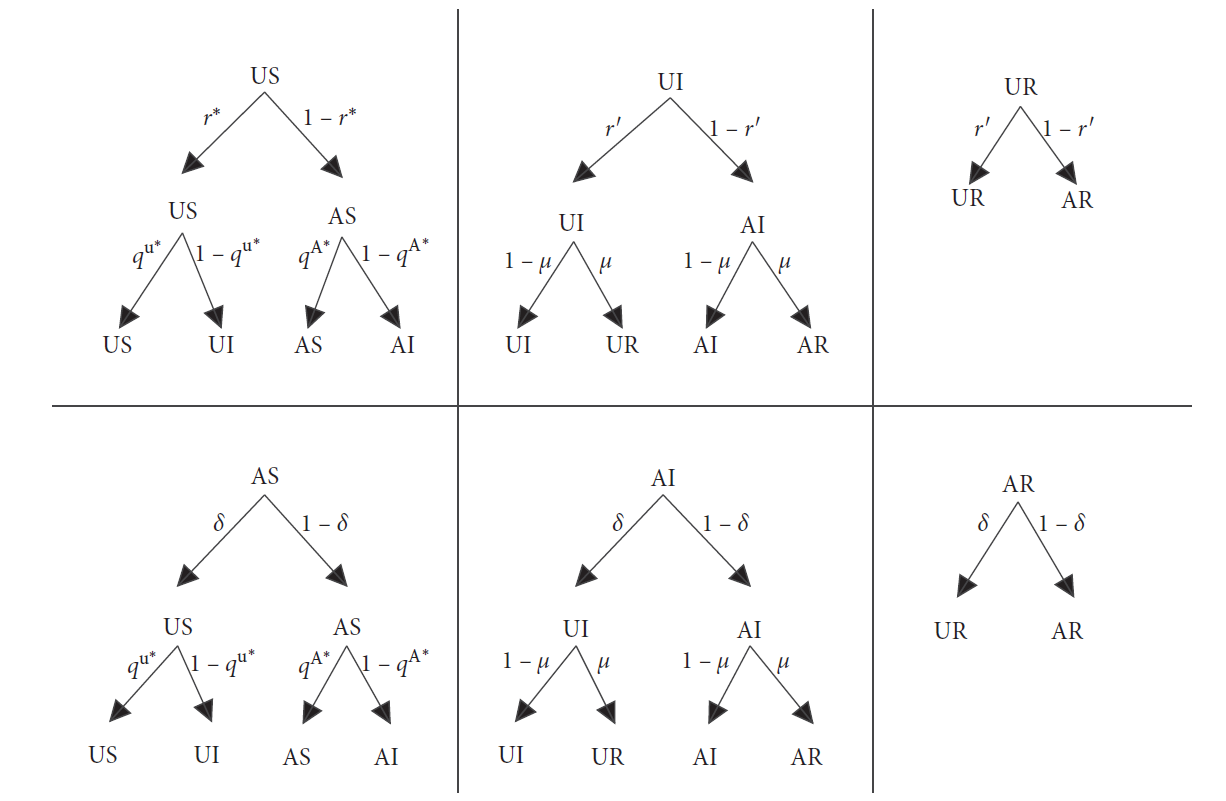
\includegraphics[width=0.6\linewidth]{0_introduction/images_review/silva2019_transition_trees}} \\
	\caption[Multiplex networks]{a) An example of a multiplex network structure resulting from the coupling of a SIR and a U-P/A-R model. b) The transition trees realized to describe the system of a SIR coupled  with a UAU model using a Markovian process. Pictures taken from articles \cite{Peng2021, Silva2019}.}
	\label{fig:sir_example3}
\end{figure}

In \cite{Peng2021}, a slightly more complex situation is described, where two possible opinions—pro-physical distancing (P) and anti-physical distancing (A)—are considered. In contrast, \cite{Frieswijk_2022} studies a simpler structure, where a SIS model is coupled with either adopting or not adopting self-protective measures.

Interesting results derived from these works include: 
\begin{itemize} 
	\item The observation of the influence of opinions on transmission speed and the final epidemic size \cite{Peng2021}. 
	\item The effect of authoritative information, publicizing epidemic prevention processes, and encouraging reasonable behavior, such as isolating when infected \cite{Zuo_2021}. 
	\item The importance of self-awareness as a mechanism to reduce disease prevalence \cite{Silva2019}. 
\end{itemize}

Finally, the experiments conducted in \cite{Frieswijk_2022} provide a stability analysis of the equilibria and explicitly calculate the epidemic threshold. Figure \ref{fig:stability_friesjiw} shows their simulations, which vary a parameter modeled as risk perception. They observe its role in the occurrence of periodic oscillations and identify a set of conditions that lead to global convergence to such a periodic solution. This is an important result, demonstrating that during an epidemic outbreak, there is a collective behavioral response, and it specifies under which conditions the situation evolves into a stable dynamic or not.

\begin{figure}[h]
	\centering
	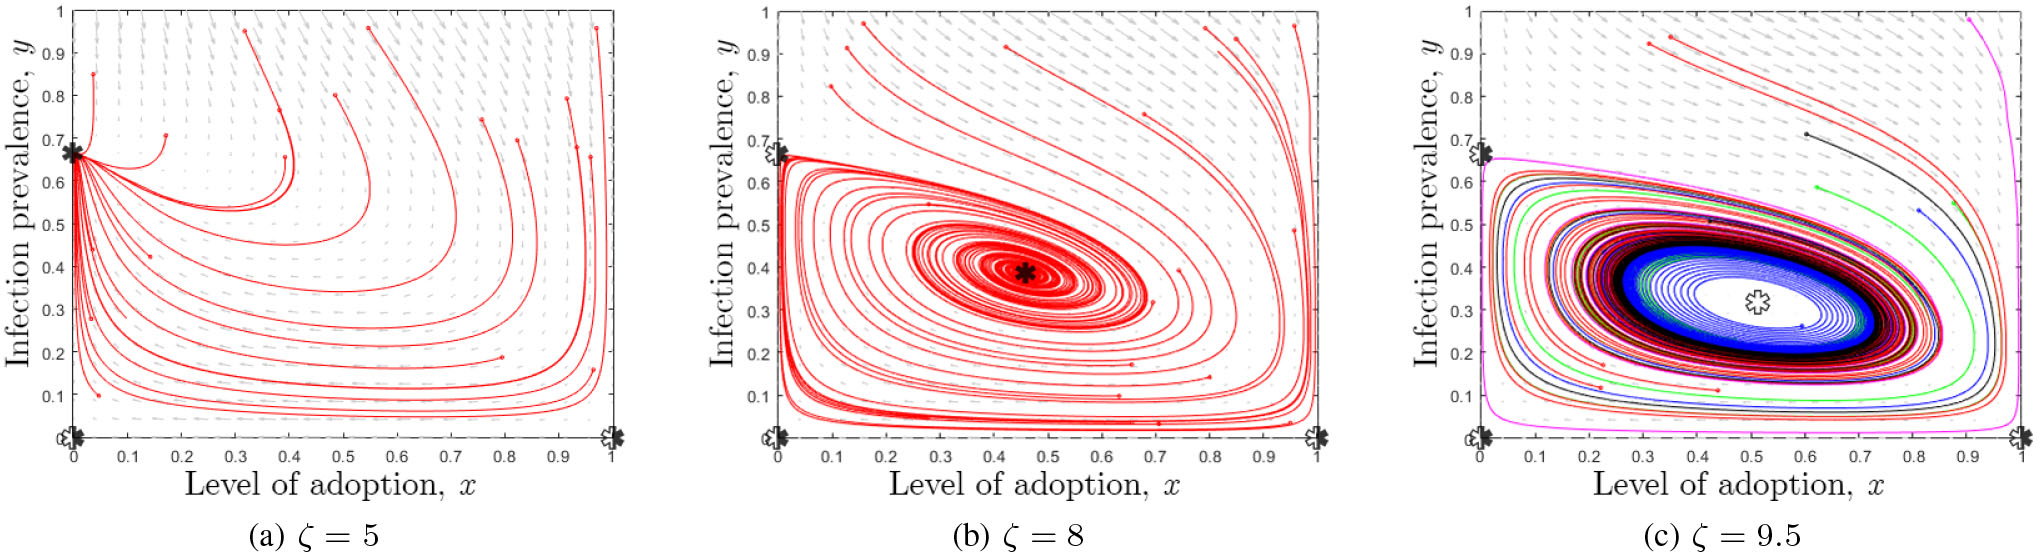
\includegraphics[width=0.95\linewidth]{0_introduction/images_review/stable_unstable_equilibria_friejs}
	\caption[Stability analysis of epi-behavior model]{Simulations taken from the article \cite{Frieswijk_2022} That show of their model evolve for different values of the risk perception parameter. Stable equilibria, saddle points and unstable equilibria are marked with a black, black-white and white asterisk, respectively.}
	\label{fig:stability_friesjiw}
\end{figure}

\subsubsection{Game theoretical models}
In the probabilistic framework, another area involves the use of game theory principles. These are used to explore strategic interactions between individuals, where participants act to maximize their utility, potentially influencing the actions of others. The concept of Nash Equilibrium is also important in this context. It is defined as "a set of strategies such that no player has an incentive to unilaterally deviate from the present strategy" \cite{Wang_2015_review}. That is, the Nash Equilibrium leads individuals to adopt strategies consistent with their goal of maximizing their benefit or utility in a perfectly rational way, forming the best responses to one another.

Many articles use this idea to model how populations adjust their behavior during an epidemic. One such example is  \cite{Auld_2003}, which focuses on the behavior of a population deciding between their sexual habits and the risk of HIV infection. The main result is derived by observing how population behavior changes as information about a possible vaccine spreads. Optimistic news lead to a decrease in the number of contacts, while pessimistic forecasts cause an increase in risky behavior, even at the same level of risk. A particularly interesting conclusion is that focusing public health messaging on dire forecasts may unintentionally lead to an increase in risky behavior.

\begin{figure}[h]
	\centering
	\subfloat[][\emph{}]
	{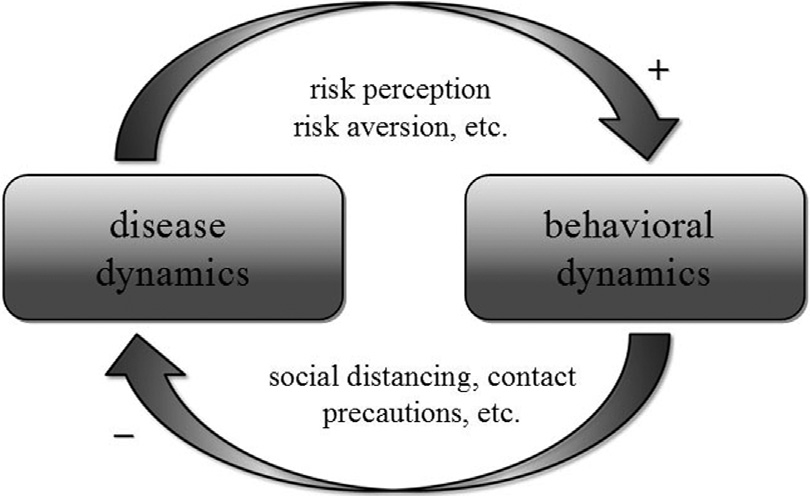
\includegraphics[width=0.38\linewidth]{0_introduction/images_review/disease_behavior_interaction_wang2015}} \quad
	\subfloat[][\emph{}]
	{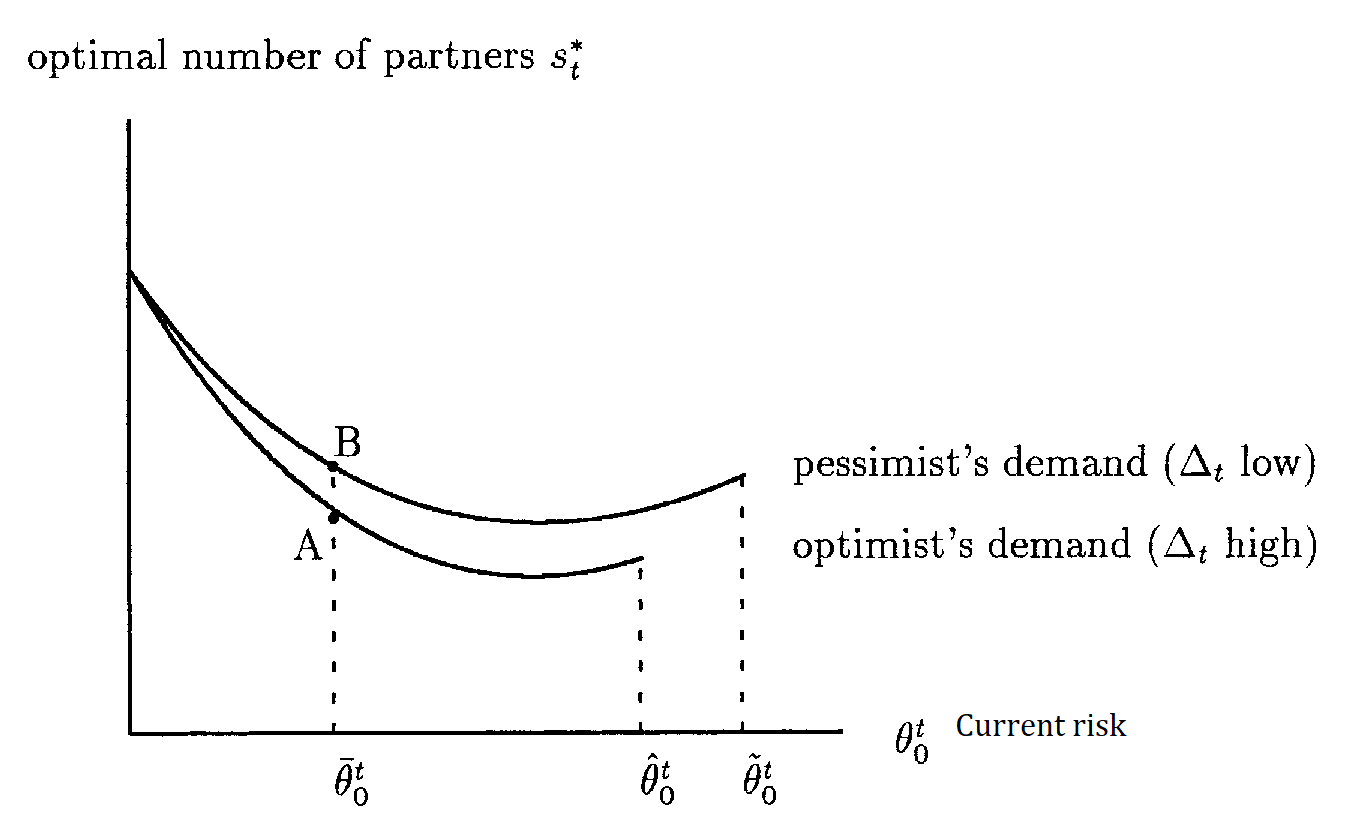
\includegraphics[width=0.58\linewidth]{0_introduction/images_review/risk_forecast_auld}} \\
	\caption[Game theory]{a) A representation of the feedback loop, taken from the article of \cite{Wang_2015}, representing the trade-off between: advantages related to avoid the disease and social cost of behave using precautions.  b) The effect on people's behavior due to optimistic or pessimistic forecasts is described in the illustration presented in \cite{Auld_2003}. The population tends to act more cautiously if there is hope that the situation will improve in the future.}
	\label{fig:abm_game}
\end{figure}

A different focus is the one that the article  \cite{Gosak_2021_game} has. Here, the behavioral change related to contact rate and especially social distancing, in the context of a pandemic situation like COVID-19  is studied to understand the efficacy of policies for partial or full voluntarily contact reduction. They aim to realize more insight into the percentage of adoption from the population of social distancing policies because increasing the quality of these estimations matters in the planning of strategies to handle a pandemic from a government point of view.

Another case study is \cite{Nunner2021}, which defines different utility functions to model the trade-off between social well-being from maintaining connections, the fatigue of doing so, and the potential physical harm those connections may cause. The main results outlined in \cite{Nunner2021} confirm that a higher number of connections between individuals leads to greater disease transmission, resulting in more infections and a shorter epidemic duration. It also highlights that "the higher the (perceived) risks of a disease, the lower the net benefit of a tie, the stronger the social distancing, and consequently the smaller the epidemic size."
Using this co-evolutionary approach, a highly correlated dynamic between the two layers emerges: a feedback loop between the spread of infection and behavioral adaptation, with structural modifications in the network occurring in the simulated scenarios.
The introduction of network-based modeling further develops this work and leads to several key findings. First, including the benefit of social connection creates multiple transmission routes for the disease. Second, a reduction in the final epidemic size only occurs when the indirect benefits are relatively low and the costs of maintaining ties are high. Finally, small changes in social behavior can have large impacts on the epidemic.
In the next paragraph, other similar studies that incorporate network models will be discussed. However, before that, a final case where the game-theoretical approach is often applied will be presented: vaccination. Many models examine the decision-making process behind vaccination, highlighting the trade-off between the benefits of getting vaccinated and the risks associated with it.
In terms of modeling, the link between behavior and epidemic spread in this case is that individuals who choose vaccination are removed from the susceptible group, with a percentage reflecting the vaccine's efficacy, thereby reducing the potential for disease transmission. In the study developed in \cite{Bauch_2012_game}, a feedback loop is established between disease prevalence and individual strategic vaccination behavior. Their model successfully fits vaccine coverage data from both the pertussis and MMR vaccine scares and can also predict future trends in disease prevalence and vaccine coverage. 
Moreover, the article highlights the phenomenon for which the vaccine fear becomes more frequent as eradication goals for more vaccine-preventable diseases are approached.

\subsubsection{Network based models}
The inclusion of networks in the modeling process has gained popularity as a tool for scientists to enhance the accuracy of their models by simulating real-world connections between people. The main goal behind developing network-based models is to create a representation of society and then use it to simulate the spread of disease. A comprehensive example of this approach is presented in \cite{VanMieghem2009}, where a method is introduced to simulate scenarios such as quarantine or regional barriers that limit population movement. By adjusting network connections—reducing contacts between nodes or cutting ties between specific regions—these models effectively demonstrate the impact of interventions like lockdowns or travel restrictions on disease transmission. They also enable analysis of how containment measures affect the trajectory of an epidemic.
Works such as \cite{Tizzoni2014} also fall into this category, utilizing urban mobility patterns as a proxy for modeling epidemics. Similarly, in \cite{Carballosa_2021}, social networks are used as a proxy for connections, hypothesizing that people's behavior in maintaining social contacts is analogous to how they might behave in the context of disease transmission.
Another innovative approach involves the development of multilayer networks, such as in \cite{Turker_2023}, where the social structure of a town is recreated. Each layer represents a different environment—ranging from homes to workplaces, distinguishing between various job types, and even considering a layer for friendships. Each individual exists across multiple layers and interacts with different groups depending on their social environment. This model found that the layer associated with friendship poses the highest risk for outbreak development, due to closer interactions and lower security measures. Consequently, even a relatively low transmissibility rate ($\beta$) can lead to a significant epidemic with many susceptible individuals involved.
\begin{figure}[h]
	\centering
	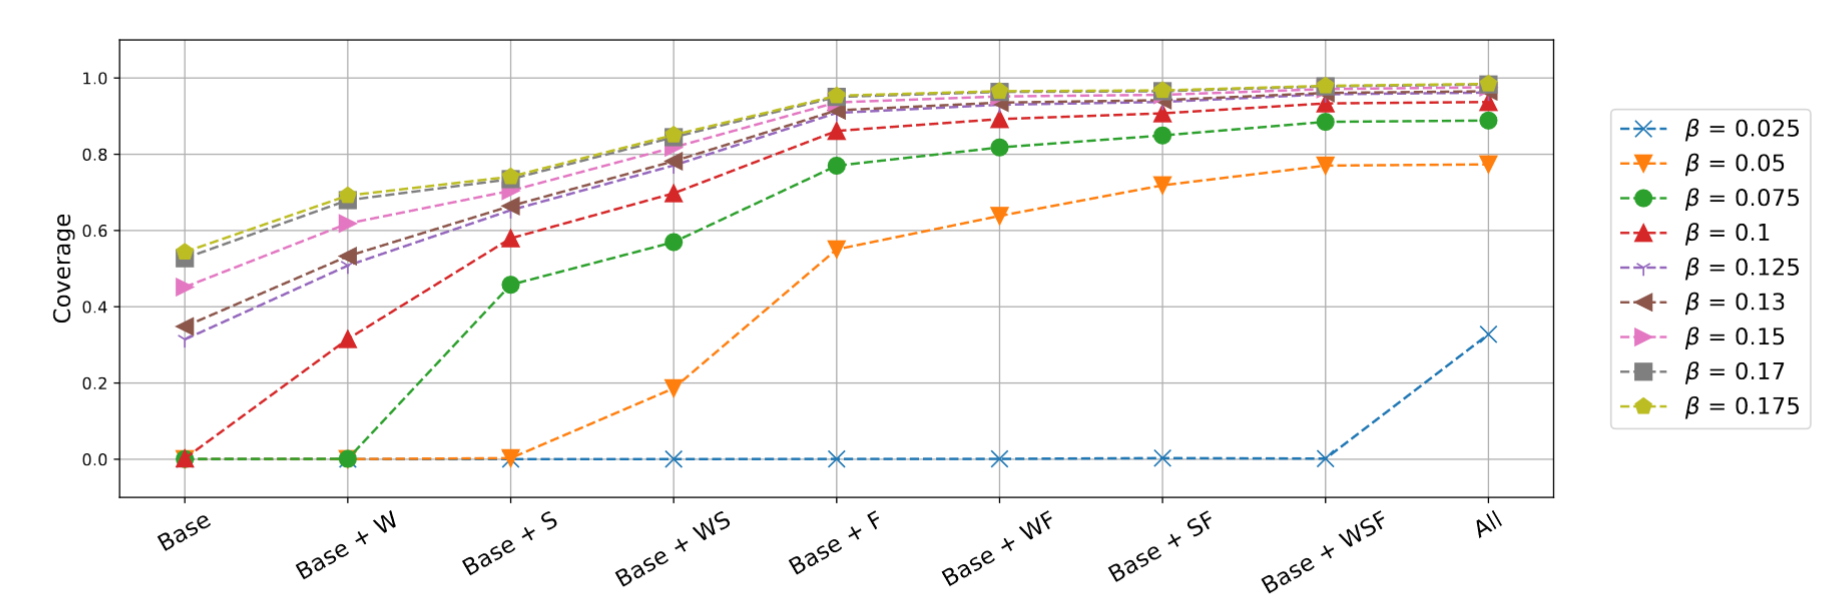
\includegraphics[width=0.9\linewidth]{0_introduction/images_review/turker_city_recreated}
	\caption[Simulation of disease spreading within a city]{In the simulation presented in \cite{Turker_2023}, a city is modeled with people divided into several social groups. They found that the layer associated with friendships is where the disease outbreak occurs with the lowest value of the infectivity parameter, $\beta$.}
	\label{fig:turkercityrecreated}
\end{figure}



\subsubsection{Threshold models}
Another possible mechanism for modeling how individuals change their actions is by observing the behaviors and opinions of their neighbors \cite{Granovetter_1978, Krassa_1988}. A well-known theoretical tool for this context is the Watts threshold model \cite{Watts_2002}, which is foundational for studying such transitions.
In \cite{Wang_2019}, various threshold models are discussed, including the Watts threshold, which is linear. In their model, each node is assigned a random threshold value based on a given distribution. The threshold represents the point at which a node changes its opinion when a certain number of its neighbors adopt a different behavior. The structure of the network is crucial for determining how opinions spread. They found that opinion propagation is most favorable in networks with low randomness and a regular structure. Additionally, they analyzed the effects of network clusters, noting that well-connected clusters can act as opinion hubs, reinforcing the spread of opinions.

\subsubsection{Ad-hoc rule-based models}
The last category of agent-based models focuses on individuals acting according to specific rules designed to simulate particular situations. A clear example of this is found in \cite{Alvarez_Zuzek_2017}, where disease propagation is modeled based on opinions for or against vaccination. The evolution of these opinions is determined by the interaction and exchange of ideas between agents and co-evolves alongside their health condition. A comprehensive set of rules is established to model all possible situations that lead to changes in both opinion and disease states. An example is visible in picture \ref{fig:alvarez_opi_vac}


\begin{figure}[h]
	\centering
	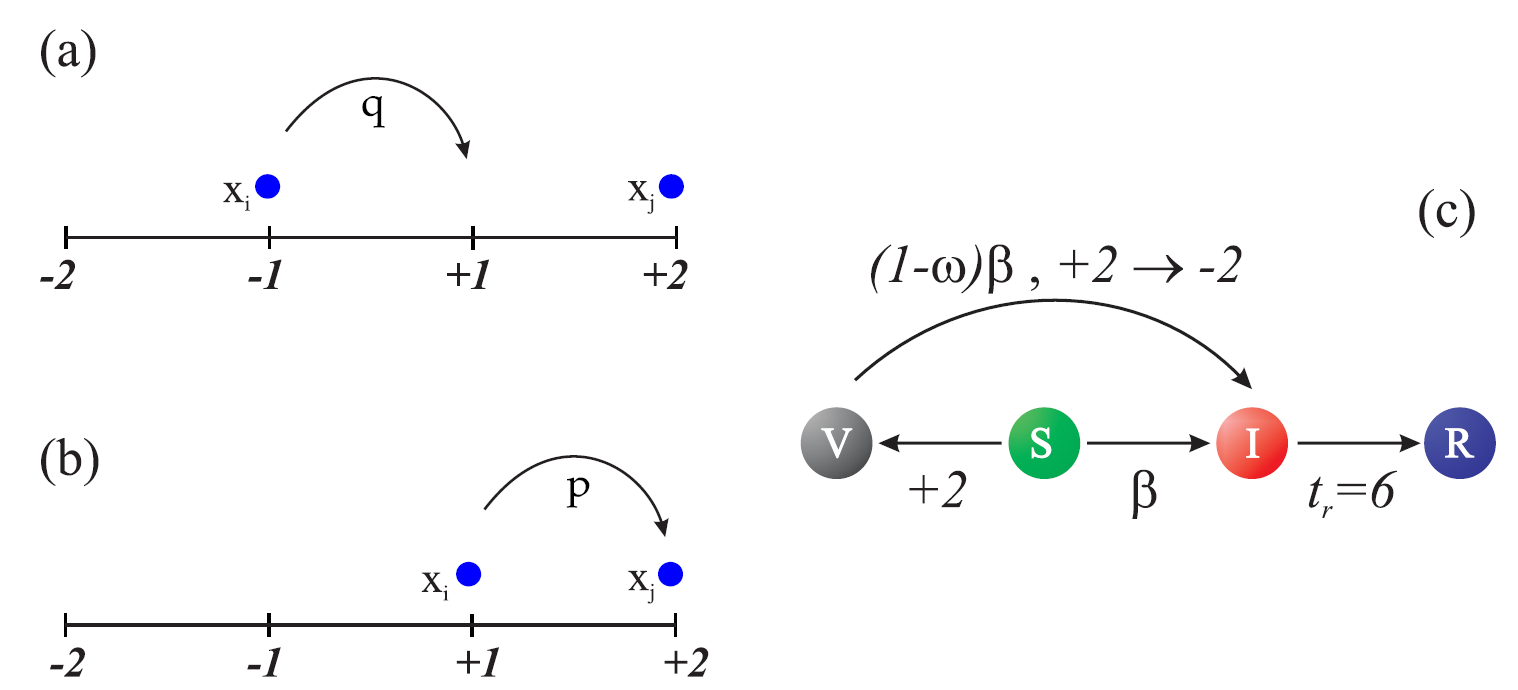
\includegraphics[width=0.8\linewidth]{0_introduction/images_review/alvarez_opi_vac}
	\caption[Rules in opinion disease model]{The picture, taken from the article \cite{Alvarez_Zuzek_2017}, illustrates the mechanisms underlying the model's dynamics. The figures on the left depict opinion dynamics: when two nodes have opposing opinions, one adjusts its state to match the other's opinion with a probability $q(a)$. If both nodes share the same opinion, the opinion is reinforced with a probability $p(b)$. The figure on the right represents contagion dynamics: a susceptible individual $S$ (green) becomes infected (red) with a probability $\beta$ and recovers (blue) after a time $t_r$. A susceptible individual can also become vaccinated $V$ (grey) upon acquiring an opinion state of $+2$. However, they can still become infected with a probability $(1-\omega) \beta$, which causes their opinion to shift to $-2$. }
	\label{fig:alvarez_opi_vac}
\end{figure}

A similar approach is developed in the article by \cite{teslya2022}, where an explicit mechanism is implemented to govern the competition between different health opinions. Individuals with a positive $+$ opinion may switch to the opposing $-$ opinion after interacting with others, following a switch rate function. By varying the parameters of this function, its behavior can become linear, saturating, or sigmoidal similar to established functions used to describe predator responses to prey population density.

Finally, the article by \cite{Collinson2014} extends the SEIR model by incorporating the effect of mass media on disease spread, using a specific set of functions. These functions account for disease prevalence, recovery rate, and media impact. The goal is to conduct a sensitivity analysis on the parameters influencing the epidemic's peak magnitude, timing, and ending. 


\subsection{Homogeneous population models}
\label{subsec:homogeneous}
This section presents the works that have most contributed to shaping the development of the thesis, the mean-field models. The assumption that the population is homogeneously mixed results in models capable of describing phenomena nationwide, which is difficult to achieve when modeling individual behavior.

However, the effectiveness of this class of models relies heavily on the modeling principles applied. Models are powerful tools, but they represent the aspects the modeler chooses to emphasize. Therefore, selecting and integrating the most promising features is crucial for creating a useful instrument. By analyzing prior works, we gain insights into what has been previously explored and the outcomes achieved.
The most interesting characteristics of various models are now presented, followed by an explanation of how they have contributed to the development of the model in this thesis.

The article \cite{Tyson_2020} was one of the first studied for its insteresting modeling approach. It integrates two dynamics: the epidemic evolution influences the parameters governing people's behavior, and, conversely, the population's behavior affects the spread of the disease. This bidirectional interaction allows for a more realistic simulation of how behavioral changes and disease dynamics influence each other.
A SIR model is associated with an opinion dynamic that occurs only within the $S$ compartment. This compartment is divided into four subgroups, representing different attitudes toward prophylactic behavior. In this way, more cautious individuals have a lower probability of becoming infected. The opinion dynamic focuses on the phenomenon of influence, modeled by a specific parameter, and on opinion amplification, a cognitive bias where confronting someone with the same belief strengthens that belief.
The most interesting aspect of their work is the concept that opinion spreads through conversation, not through a utilitarian or contagion process like fear diffusion.

A similar hypothesis of social learning is explored in the article \cite{Tanaka_2002}. In this model, both risky and cautious behaviors coexist in the population and can be transmitted. The model also incorporates the effects of clustering and the phenomenon of "cultural bias." This bias suggests that the risky trait is more likely to be adopted by cautious individuals than the reverse. Additionally, the authors introduce the concept of uncertainty regarding the infection causes, meaning that people are unsure of the best way to behave to avoid contracting the disease.


In the article \cite{Bongarti2023}, compliance with the use of NPIs (Non-Pharmaceutical Interventions) is the central focus of the behavioral component of the model. In this case, non-compliance is modeled as a social contagion: the population is divided into two groups, compliant ($c$) and non-compliant ($nc$). Using the mass-action mixing property, compliant individuals become non-compliant, but there is no recovery once their status changes. The primary goal is to understand the interplay between the stringency of lockdown measures, non-compliant behavior, and the spread of the disease.


Vaccine adoption and awareness diffusion are the main arguments developed in \cite{Zuo2022}. Awareness is present only in the Susceptible compartment, and there is a term, $M(t)$, that represents the accumulated density of awareness programs driven by various information sources. This term is influenced by several factors: awareness generated by neighboring individuals, the intensity of awareness programs in response to the prevalence of the disease, and a waning effect due to the decreasing quality or effectiveness of the information over time. Their complete model and the interplay between disease and behavior is shown in figure  \ref{fig:mean_models_1}. 
An interesting aspect of this article is that the authors evaluate their model using data from the COVID-19 vaccination campaign in China. They observe how their model effectively reproduces the population behavior and government policies during different phases of the epidemic.

\begin{figure}[h]
	\centering
	\subfloat[][\emph{}]
	{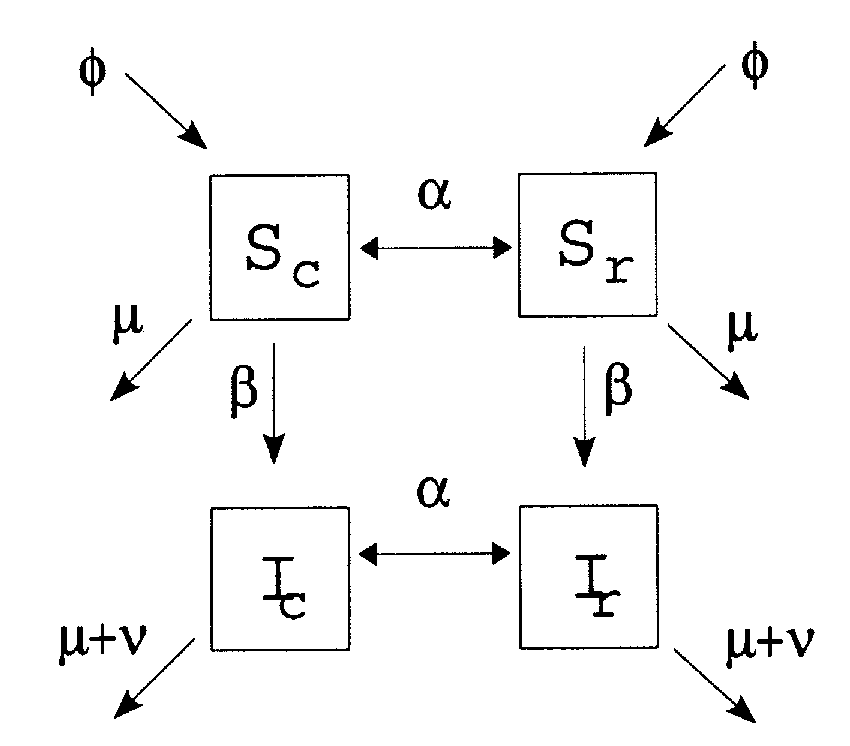
\includegraphics[width=0.35\linewidth]{0_introduction/images_review/Tanaka_model}} \quad
	\subfloat[][\emph{}]
	{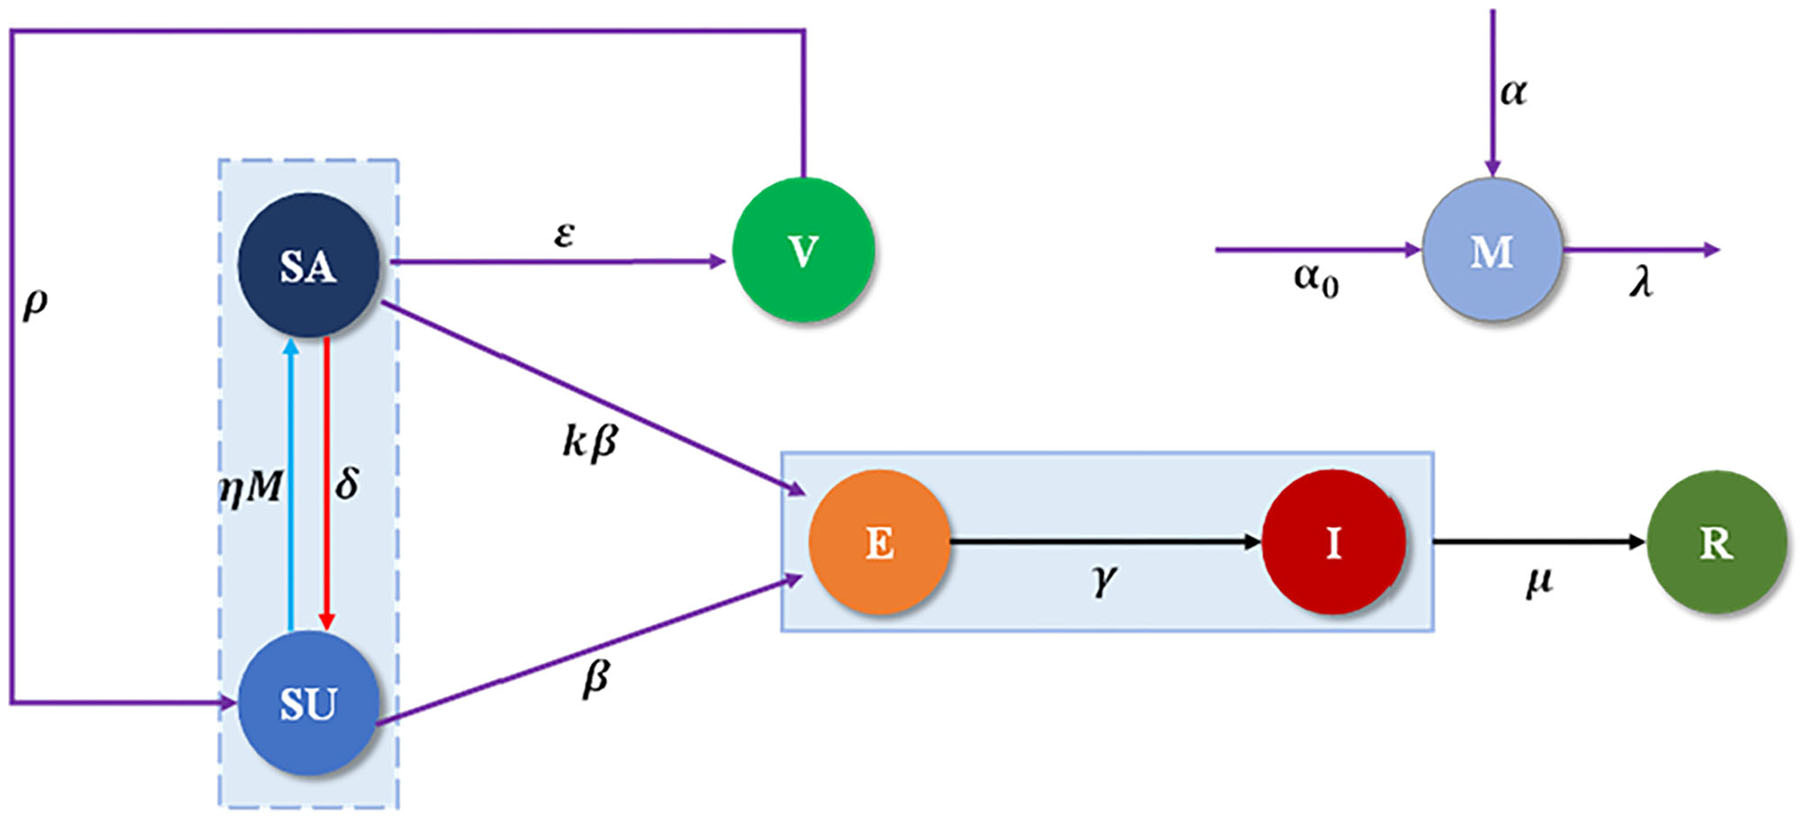
\includegraphics[width=0.6\linewidth]{0_introduction/images_review/zou_2022_SEIRVM}} \\
	\caption[Mean field models literature review]{a) The model presented in \cite{Tanaka_2002} shows horizontal layers representing behavioral diffusion, while vertical layers represent disease spread. Behavior diffuses between both infected and susceptible individuals, but this is not depicted for visual clarity. b) The model developed in \cite{Zuo2022} incorporates behavior dynamics only in the susceptible ($S$) layer, influencing both contagion rates and the probability of vaccination. The $M$ compartment follows its own dynamics, observing the state of the disease and the distribution of public opinion, and it influences the diffusion of awareness.}
	\label{fig:mean_models_1}
\end{figure}

An interesting article on the subject of behavior and vaccines is \cite{Epstein_2021}. In this model, an initially susceptible population can split into two opposing compartments, depending on what they fear more: the disease or vaccination. The model includes six compartments, with the fear dynamics occurring only in the susceptible ($S$) compartment.

In this scenario, fear of vaccination can undermine outbreak control. Initially, people may get vaccinated, but they stop too early as their fears reverse. The study also conducts a sensitivity analysis on the contact rates for the two fears, showing that transmission speed significantly affects the model’s outcomes. The results range from multiple infection waves to complete disease extinction without an outbreak, depending on the conditions.

\section{Analysis of the literature}
To conclude this chapter on the literature review, an analysis of the models discussed is presented, with a focus on how they relate to the scope and aim of this thesis. This evaluation wants to explain the key insights gained from the literature and highlight also what are the differences and novelty introduced in this work.

\subsection{Individual state models}
Referring to the models presented in the previous section \ref{subsec:individual_state}, most face the challenge of developing complex simulations to model the evolution of disease and individual behavior, but struggle to scale these simulations to the nationwide level. In many cases, small groups of agents are used, such as the 50 nodes mentioned in \cite{Nunner2021}, and even in works where a larger number of nodes is implemented, the count is typically in the thousands \cite{Granell2013}, not in the millions, as would be necessary for national-scale modeling. To overcome this difficulty, some articles use mean-field approximations, considering the limit of an infinite population size and employing statistical approaches \cite{Frieswijk_2022}.

Another critical issue these models face is the need for large amounts of data to accurately represent how populations behave during unusual situations like epidemic outbreaks. Without this data, it becomes difficult to draw precise conclusions from the models. While these models can still provide useful insights, their application for making precise, real-world predictions remains limited. They are better suited as scientific tools for exploring theoretical scenarios rather than for offering actionable advice on a larger scale. An article that demonstrates the volume of data required to test a model with real-world scenarios is \cite{Kemp_2021}. In this study, data from three different countries—Luxembourg, Austria, and Sweden—was collected, including information on total detected cases, hospitalized individuals, people in intensive care units (ICUs), and deaths. This comprehensive dataset was used to fit the model.

In the case of behavioral-epidemic models, even fewer data were available until the recent COVID-19 pandemic. As explained in \cite{Gosak2021}, this lack of data was a significant challenge. However, they show how it was partially addressed by implementing models based on population behavior with respect to influence. Despite these improvements, the availability of data today is certainly better, offering more robust insights. 

As they say: \textit{"The issue is that research has not yet provided empirical benchmarks for endogenous contact rates in disease scenarios, so it is unclear how such policies can be evaluated scientifically: ideally a policy is benchmarked against a set of counterfactuals given the disease, not compared with what was before the disease".}

\subsection{Well-mixed population models}
As stated earlier in paragraph \ref{subsec:homogeneous}, a major critique of developing complex mean-field models is that if they are not supported by consistent observation of the phenomena they aim to reproduce, their capacity to generate meaningful insights can be significantly limited. For this reason, proper empirical grounding is one of the main objectives pursued in this thesis work. The comparison of the model's emerging dynamics with real-world data is a reliable method to test the model's validity and evaluate its predictive capacity.
Reading through works in this field, a common approach emerges for modeling systems that aim to incorporate two distinct dynamics, such as behavior and disease spread. Most of these models introduce additional compartments, which represent subgroups of homogeneously mixed individuals sharing common characteristics—typically, their disease state and course of action. The primary distinction lies in how modelers handle the flow between these compartments: while some works focus on the influence of behavior solely within the Susceptible layer \cite{Epstein_2021, Tyson_2020, Zuo2022}, others implement a full double-layer model \cite{Bongarti2023, Bulai2023, Tanaka_2002}. Another key difference is whether the change in behavior dynamics is unidirectional, as in \cite{Bongarti2023}, or bidirectional, as seen in \cite{Epstein_2021, Tyson_2020, Tanaka_2002, Zuo2022}, where individuals can adjust their actions in both directions.
Notably, some of the most influential aspects drawn from the literature for this thesis include the "double fear" structure developed by \cite{Epstein_2021} and the awareness element that influences behavior change, modeled through an external node $M(t)$ in \cite{Zuo2022}. Additionally, this thesis seeks to implement a fully coupled double-layer model for behavior and epidemic spread, incorporating elements such as memory waning and fatigue, which combine with conversational mechanisms to create bidirectional flows in the behavioral model.
Unlike \cite{Tanaka_2002}, which uses a simpler epidemic model, this work employs a more complex one to accurately reflect COVID-19 data. Furthermore, the models developed in \cite{Bulai2023} and \cite{Smaldino_2021} share structural similarities with this thesis. However, \cite{Bulai2023} assumes faster information diffusion than disease transmission, decoupling the two layers, while \cite{Smaldino_2021} focuses on homophily and polarization of compartments—factors not considered here due to data limitations.
The following chapter will explain the development of the model, integrating the features and ideas here presented.

